% ====================================================================================
\chapter{深度学习：从拉格朗日乘子到神经网络}
% ====================================================================================

\section*{引言：让机器学会"看"}

\marginnote{\textbf{深度学习三巨头}：Geoffrey Hinton、Yann LeCun、Yoshua Bengio因``深度学习的突破性贡献''共同获得2018年图灵奖（计算机界的诺贝尔奖）。2012年Hinton学生的AlexNet在ImageNet竞赛中取得突破，标志着深度学习时代的开始。}

\marginnote{\textbf{图灵奖}以计算机科学之父Alan Turing命名，是计算机界最高荣誉。图灵(1912--1954)提出了图灵机概念，奠定了现代计算机理论基础。他在二战中破解了纳粹密码，却因同性恋被迫害，最终服毒自杀。2009年英国政府正式道歉，2013年英女王宣布对其赦免。}

想象一个问题：如何让计算机识别手写数字？

给计算机一张 $28 \times 28$ 像素的灰度图片（共784个数字，每个数字表示一个像素的亮度），它需要输出 0-9 中的某个答案。

\textbf{传统方法}是人工设计规则：``6有一个圈''、``7有一横一竖''。但这种方法太脆弱——字迹潦草一点就失效了。

\textbf{深度学习的思路}完全不同：我们不告诉计算机规则，而是给它大量``图片-答案''的配对数据，让它\textbf{自己从数据中学出}识别规则。

这听起来很神奇，但数学上，它不过是一个\textbf{带约束的优化问题}——正是我们前几章学过的内容。
\storynote{Rumelhart、Hinton 与 Williams}{1986年，三人在 Nature 上发表了一篇只有四页的短文《Learning representations by back-propagating errors》，"反向传播"从此家喻户晓。但同样的公式，控制论学者早在1960年代就用来算火箭轨迹的灵敏度——第8章的伴随方程。本章要讲的，正是这段被遗忘的血缘。}

\vspace{0.3cm}
\noindent\textit{为什么一个有上亿参数的网络，算一次梯度只比算一次输出贵两三倍？为什么"反向传播"要从最后一层往回算，而不是从第一层往前算？为什么控制论里算火箭轨迹灵敏度的公式，和训练神经网络的公式一模一样？}

\begin{quote}
\textbf{本章目标}：用拉格朗日乘子法的视角，理解深度学习的数学本质。你会发现，神经网络的``反向传播''算法，正是约束优化中伴随方程的离散版本。
\end{quote}

\begin{tcolorbox}[colback=green!5, colframe=green!60!black, title=学完这章，你将能够...]
\begin{itemize}
    \item 手推一个两层神经网络的前向和反向传播
    \item 解释梯度消失/爆炸的数学原因（见扩展阅读）
    \item 用自己写的自动微分引擎训练一个小型分类器（编程题）
    \item 理解为什么反向传播是伴随方法的离散版本
    \item 分析激活函数、损失函数的选择依据（见扩展阅读）
\end{itemize}
\end{tcolorbox}

\begin{insightbox}
\textbf{阅读本章前，请确保你理解}：
\begin{itemize}
    \item 拉格朗日乘子法的基本思想（第1章：把约束融入目标函数）
    \item 约束优化的KKT条件（第1章：最优解满足的必要条件）
    \item （推荐）伴随方程的直觉（第8章：从未来往回算影响）
\end{itemize}

\textbf{如果你跳过了前面的章节}，至少要理解这个核心思想：
\begin{center}
\fbox{\parbox{0.85\textwidth}{
拉格朗日乘子 $\lambda$ 的含义：如果约束放松一点点，目标函数会变化多少？\\[0.2em]
这个``影子价格''的概念，在神经网络中变成了``误差信号''。
}}
\end{center}
\end{insightbox}

% ------------------------------------------------------------------------------------
\section{从函数逼近到神经网络}

\subsection{问题的数学表述}

识别手写数字，本质上是要找到一个函数：
\begin{equation}
f: \mathbb{R}^{784} \to \{0, 1, \ldots, 9\}
\end{equation}

输入是784维向量（图片的像素值），输出是一个类别标签。

但这样的函数有无穷多个，我们怎么找到``正确''的那个？答案是：\textbf{用数据来约束}。

假设我们有 $N$ 个训练样本 $\{(x^{(k)}, y^{(k)})\}_{k=1}^N$，其中 $x^{(k)}$ 是第 $k$ 张图片，$y^{(k)}$ 是对应的真实标签。我们希望找到的函数 $f$ 能够在这些样本上表现良好：
\begin{equation}
f(x^{(k)}) \approx y^{(k)}, \quad k = 1, \ldots, N
\end{equation}

\subsection{参数化函数族}

直接在所有函数中搜索是不现实的。深度学习的策略是：选定一个\textbf{参数化的函数族}，然后在这个族里搜索最优参数。

最简单的参数化函数是线性函数：$f(x) = Wx + b$，其中 $W$ 是权重矩阵，$b$ 是偏置向量。但线性函数的表达能力太弱，无法捕捉复杂的模式。

\textbf{神经网络}的想法是：把多个简单的非线性函数\textbf{复合}起来，形成一个复杂的函数。

\begin{definition}[神经网络]
一个 $n$ 层神经网络是如下形式的复合函数：
\begin{equation}
f(x; \theta) = f_n \circ f_{n-1} \circ \cdots \circ f_2 \circ f_1(x)
\end{equation}
其中每一层 $f_i$ 通常具有如下形式：
\begin{equation}
f_i(z; W_i, b_i) = \sigma(W_i z + b_i)
\end{equation}
这里：
\begin{itemize}
    \item $W_i \in \mathbb{R}^{d_{i} \times d_{i-1}}$ 是第 $i$ 层的\textbf{权重矩阵}
    \item $b_i \in \mathbb{R}^{d_i}$ 是第 $i$ 层的\textbf{偏置向量}
    \item $\sigma: \mathbb{R} \to \mathbb{R}$ 是\textbf{激活函数}（非线性函数），逐元素作用
    \item $\theta = \{W_1, b_1, \ldots, W_n, b_n\}$ 是所有待学习的参数
\end{itemize}
\end{definition}

\begin{figure}[h]
\centering
\begin{tikzpicture}[node distance=2cm, >=stealth]
    % 输入层
    \node[circle, draw, minimum size=0.8cm] (x1) at (0, 1.5) {$x_1$};
    \node[circle, draw, minimum size=0.8cm] (x2) at (0, 0) {$x_2$};
    \node[circle, draw, minimum size=0.8cm] (x3) at (0, -1.5) {$x_3$};
    \node[below=0.3cm of x3] {输入层};
    
    % 隐藏层1
    \node[circle, draw, fill=blue!10, minimum size=0.8cm] (h11) at (3, 1) {$z_1^{(1)}$};
    \node[circle, draw, fill=blue!10, minimum size=0.8cm] (h12) at (3, -1) {$z_2^{(1)}$};
    \node[below=0.3cm of h12] {隐藏层};
    
    % 输出层
    \node[circle, draw, fill=green!10, minimum size=0.8cm] (y) at (6, 0) {$y$};
    \node[below=0.3cm of y] {输出层};
    
    % 连接
    \foreach \i in {1,2,3} {
        \foreach \j in {1,2} {
            \draw[->] (x\i) -- (h1\j);
        }
    }
    \draw[->] (h11) -- (y);
    \draw[->] (h12) -- (y);
    
    % 标注
    \node[above right=0.1cm of x1, font=\small] {$W_1, b_1$};
    \node[above right=0.1cm of h11, font=\small] {$W_2, b_2$};
\end{tikzpicture}
\caption{一个两层神经网络的结构。每条边代表一个权重，信息从左向右流动。}
\end{figure}

\subsection{为什么需要非线性？}

\begin{theorem}[线性函数复合的退化性]
多个线性函数的复合仍然是线性函数。具体地，如果 $f_i(z) = W_i z$，则：
\begin{equation}
f_n \circ \cdots \circ f_1(x) = W_n W_{n-1} \cdots W_1 x = W' x
\end{equation}
其中 $W' = W_n W_{n-1} \cdots W_1$ 仍是一个矩阵。
\end{theorem}

这意味着，如果没有非线性激活函数 $\sigma$，无论堆叠多少层，神经网络的表达能力都等价于单层线性变换。非线性是深度网络表达能力的来源。

\begin{definition}[常用激活函数]
\begin{itemize}
    \item \textbf{ReLU}（Rectified Linear Unit）：$\sigma(x) = \max(0, x)$
    \item \textbf{Sigmoid}：$\sigma(x) = \frac{1}{1 + e^{-x}}$
    \item \textbf{Tanh}：$\sigma(x) = \frac{e^x - e^{-x}}{e^x + e^{-x}}$
\end{itemize}
\end{definition}

\marginnote{ReLU因其计算简单且能缓解``梯度消失''问题，成为现代深度学习中最常用的激活函数。它的导数在正半轴恒为1，使得梯度能够有效传播。}

% ------------------------------------------------------------------------------------
\section{学习即优化}

\subsection{损失函数}

有了参数化的函数族，下一步是定义``什么是好的参数''。我们需要一个\textbf{损失函数}（Loss Function）来度量预测与真实值的差距。

给定训练数据 $\{(x^{(k)}, y^{(k)})\}_{k=1}^N$，定义总损失：
\begin{equation}
L(\theta) = \frac{1}{N} \sum_{k=1}^N \ell\big(f(x^{(k)}; \theta), \, y^{(k)}\big)
\end{equation}

其中 $\ell(\hat{y}, y)$ 是单个样本的损失。常用的损失函数包括：

\begin{itemize}
    \item \textbf{均方误差}（用于回归）：$\ell(\hat{y}, y) = \frac{1}{2}\|\hat{y} - y\|^2$
    \item \textbf{交叉熵}（用于分类）：$\ell(\hat{y}, y) = -\sum_c y_c \log \hat{y}_c$
\end{itemize}
\clarify{还记得第6章吗？交叉熵损失就是最小化预测分布和真实分布的KL散度。选择交叉熵不是拍脑袋决定的，而是信息论的必然结论！}

\subsection{优化问题}

训练神经网络就是求解：
\begin{equation}
\min_\theta L(\theta) = \min_\theta \frac{1}{N} \sum_{k=1}^N \ell\big(f(x^{(k)}; \theta), \, y^{(k)}\big)
\end{equation}

这是一个\textbf{无约束优化问题}。最直接的方法是梯度下降：
\begin{equation}
\theta^{(t+1)} = \theta^{(t)} - \eta \nabla_\theta L(\theta^{(t)})
\end{equation}

其中 $\eta > 0$ 是学习率。

\textbf{核心问题}：如何高效计算梯度 $\nabla_\theta L$？

现代神经网络动辄有数百万甚至数十亿参数，直接用有限差分计算梯度（对每个参数扰动一下，观察损失变化）是不现实的。我们需要一种高效的方法。
\think{有限差分要算多少次前向？$P$ 个参数就要 $P+1$ 次。GPT-3 有 1750 亿个参数——每算一次梯度就要跑 1750 亿次前向传播。反向传播只要"一次前向 + 一次反向"。这就是本章要解释的奇迹。}

% ------------------------------------------------------------------------------------
\section{计算图：约束优化的视角}

这里是本章的核心洞察：\textbf{把神经网络的计算过程看作一个约束优化问题}。

\subsection{展开复合函数}

考虑一个简单的三层网络。原始写法是：
\begin{equation}
L = \ell\big(f_3(f_2(f_1(x)))\big)
\end{equation}

现在，我们引入\textbf{中间变量}：
\begin{align}
z_1 &= f_1(x; \theta_1) \\
z_2 &= f_2(z_1; \theta_2) \\
z_3 &= f_3(z_2; \theta_3) \\
L &= \ell(z_3)
\end{align}

\textbf{关键观察}：每个等式 $z_i = f_i(z_{i-1}; \theta_i)$ 都是一个\textbf{约束条件}！

\subsection{约束优化形式}

\begin{keyformula}[title=神经网络训练的约束优化形式]
\textbf{原始问题}（无约束形式）：
\begin{equation}
\min_\theta \ell\big(f_n(\cdots f_2(f_1(x; \theta_1); \theta_2) \cdots; \theta_n)\big)
\end{equation}

\textbf{等价问题}（约束形式）：
\begin{equation}
\begin{aligned}
\min_{\theta, z_1, \ldots, z_n} \quad & \ell(z_n) \\
\text{s.t.} \quad & z_1 = f_1(x; \theta_1) \\
& z_2 = f_2(z_1; \theta_2) \\
& \quad \vdots \\
& z_n = f_n(z_{n-1}; \theta_n)
\end{aligned}
\end{equation}
\end{keyformula}

\begin{tcolorbox}[colback=yellow!10, colframe=orange!80, title=本章的核心观点]
\textbf{深度学习不是什么新东西——它就是第1章的拉格朗日乘子法，只是约束变成了一串"级联"的等式 $z_i = f_i(z_{i-1}; \theta_i)$——每一层网络一条。}对每条约束引入乘子 $\lambda_i$，一阶条件自动给出反向传播。

\begin{center}
\renewcommand{\arraystretch}{1.3}
\small
\begin{tabular}{llll}
\toprule
 & \textbf{第1章} & \textbf{第8章（离散）} & \textbf{本章} \\
\midrule
变量 & $x$ & 状态 $x_k$、控制 $u_k$ & 层输出 $z_i$、参数 $\theta_i$ \\
目标 & $f(x)$ & $\sum_k L_k + \phi(x_N)$ & 损失 $\ell(z_n)$ \\
约束 & $g(x) = 0$ & $x_{k+1} = f(x_k, u_k)$ & $z_i = f_i(z_{i-1}; \theta_i)$ \\
乘子 & $\lambda$ & $\lambda_k$（协态） & $\lambda_i$（误差信号 $\delta_i = -\lambda_i$） \\
一阶条件 & $\nabla f + \lambda^\top \nabla g = 0$ & $\lambda_k = (\partial f/\partial x_k)^\top \lambda_{k+1} - (\partial L_k/\partial x_k)^\top$ & $\lambda_i = (\partial f_{i+1}/\partial z_i)^\top \lambda_{i+1}$ \\
影子价格 & $-df^*/d\epsilon$ & $-\partial J/\partial x_k$ & $-\partial L/\partial z_i$ \\
\bottomrule
\end{tabular}
\end{center}
这不是巧合：反向传播不是从天上掉下来的，而是把"每层一条约束"交给乘子法之后自然涌现的。
\end{tcolorbox}
\review{第8章}{把第8章的离散轨迹优化并排放在这里：状态 $x_k$ $\leftrightarrow$ 层输出 $z_i$，控制 $u_k$ $\leftrightarrow$ 参数 $\theta_i$，动力学 $x_{k+1} = f(x_k, u_k)$ $\leftrightarrow$ 层 $z_i = f_i(z_{i-1}; \theta_i)$，终端代价 $\phi(x_N)$ $\leftrightarrow$ 损失 $\ell(z_n)$。第8章"伴随方程：反向传播的原型"一节已经把答案写好了。}

这就是一个\textbf{带等式约束的优化问题}——和第1章学的完全一样，只是约束变成了一系列级联的等式。
\think{对比第3章的变分法：那里约束是$y_{k+1} - y_k = v_k \Delta x$，这里约束是$z_{i+1} = f_{i+1}(z_i)$。结构完全一样！神经网络是变分法的离散版本。}

\begin{figure}[h]
\centering
\begin{tikzpicture}[node distance=2.2cm, >=stealth]
    \node[circle, draw, thick] (x) {$x$};
    \node[circle, draw, thick, fill=blue!10, right of=x] (z1) {$z_1$};
    \node[circle, draw, thick, fill=blue!10, right of=z1] (z2) {$z_2$};
    \node[circle, draw, thick, fill=blue!10, right of=z2] (z3) {$z_3$};
    \node[circle, draw, thick, fill=red!10, right of=z3] (L) {$L$};

    \draw[->, thick] (x) -- node[above, font=\small] {$f_1(\cdot; \theta_1)$} (z1);
    \draw[->, thick] (z1) -- node[above, font=\small] {$f_2(\cdot; \theta_2)$} (z2);
    \draw[->, thick] (z2) -- node[above, font=\small] {$f_3(\cdot; \theta_3)$} (z3);
    \draw[->, thick] (z3) -- node[above, font=\small] {$\ell$} (L);

    \node[below=0.5cm of z1, font=\small, text=gray] {约束1};
    \node[below=0.5cm of z2, font=\small, text=gray] {约束2};
    \node[below=0.5cm of z3, font=\small, text=gray] {约束3};
\end{tikzpicture}
\caption{计算图：每个节点是一个变量，每条边对应一个约束}
\end{figure}

% ------------------------------------------------------------------------------------
\section{拉格朗日函数与伴随变量}

\subsection{构造拉格朗日函数}
\review{第1章}{拉格朗日乘子法的核心：对每个约束$g_i(x)=0$引入乘子$\lambda_i$，构造$\mathcal{L} = f + \sum_i \lambda_i g_i$。乘子的值告诉你"放松约束能获得多少好处"。}

按照第1章的方法，对每个约束引入拉格朗日乘子：

\begin{keyformula}[title=神经网络的拉格朗日函数]
\begin{equation}
\mathcal{L}(\theta, z, \lambda) = \ell(z_n) + \sum_{i=1}^n \lambda_i^\top \big(z_i - f_i(z_{i-1}; \theta_i)\big)
\end{equation}

其中 $\lambda_i \in \mathbb{R}^{d_i}$ 是约束 $z_i = f_i(z_{i-1}; \theta_i)$ 对应的拉格朗日乘子。
\end{keyformula}

\marginnote{注意：这里我们约定 $z_0 = x$（输入）。每个 $\lambda_i$ 的维度与 $z_i$ 相同。}

\subsection{驻点条件（KKT条件）}

在最优点，拉格朗日函数对所有变量的偏导数为零。

\textbf{对 $z_i$ 求导}（$i < n$）：

$z_i$ 出现在两个地方：第 $i$ 个约束项 $\lambda_i^\top z_i$ 和第 $i+1$ 个约束项 $-\lambda_{i+1}^\top f_{i+1}(z_i; \theta_{i+1})$。因此：
\begin{equation}
\frac{\partial \mathcal{L}}{\partial z_i} = \lambda_i - \left(\frac{\partial f_{i+1}}{\partial z_i}\right)^\top \lambda_{i+1} = 0
\end{equation}

\textbf{对 $z_n$ 求导}（最后一层）：

$z_n$ 出现在损失项 $\ell(z_n)$ 和约束项 $\lambda_n^\top z_n$ 中：
\begin{equation}
\frac{\partial \mathcal{L}}{\partial z_n} = \nabla \ell(z_n) + \lambda_n = 0 \quad \Rightarrow \quad \lambda_n = -\nabla \ell(z_n)
\end{equation}

整理这些条件，我们得到：

\begin{keytheorem}[title=伴随方程（反向传播公式）]
\begin{equation}
\boxed{
\begin{aligned}
\lambda_n &= -\nabla \ell(z_n) \quad \text{（终端条件）} \\[5pt]
\lambda_i &= \left(\frac{\partial f_{i+1}}{\partial z_i}\right)^\top \lambda_{i+1}, \quad i = n-1, \ldots, 1 \quad \text{（递推公式）}
\end{aligned}
}
\end{equation}

这正是深度学习中著名的\textbf{反向传播算法}！
\end{keytheorem}

\begin{physicalmeaning}
$\lambda_i$ 的意义是什么？

回忆第1章：拉格朗日乘子 $\lambda$ 表示``如果约束放松一点，目标函数会变化多少''——即约束的\textbf{影子价格}。

在神经网络中，$\lambda_i = -\frac{\partial L}{\partial z_i}$ 表示：如果第 $i$ 层的输出 $z_i$ 变化一点，最终损失 $L$ 会变化多少。

这就是为什么深度学习文献中常把 $\delta_i = -\lambda_i$ 称为``误差信号''——它告诉我们每一层对最终误差的``贡献''。

一句话总结：本章的约束是"每一层的输出必须等于上一层输出经过这一层的结果"；乘子 $\lambda_i$ 是第 $i$ 层输出的影子价格——偷偷把 $z_i$ 改一点，最终损失会变多少（差一个负号）。反向传播就是从最后一层往回算所有影子价格。
\end{physicalmeaning}
\clarify{符号约定：本书从第1章起写 $\Lag = f + \lambda^\top g$，因此 $\lambda$ 等于"目标对约束松弛量导数"的相反数（第1章 $\lambda = -df^*/d\epsilon$）。本章的 $\lambda_i = -\partial L/\partial z_i$ 与第8章离散伴随方程的 $\lambda_N = -\partial\phi/\partial x_N$ 都遵守这一约定；深度学习文献中的 $\delta_i = \partial L/\partial z_i$ 只差一个负号。}

\subsection{参数梯度}

有了 $\lambda_i$，计算参数梯度就很简单了。

对 $\theta_i$ 求导：
\begin{equation}
\frac{\partial \mathcal{L}}{\partial \theta_i} = -\lambda_i^\top \frac{\partial f_i}{\partial \theta_i}
\end{equation}

由于 $\lambda_i = -\frac{\partial L}{\partial z_i}$，我们有：
\begin{equation}
\boxed{\frac{\partial L}{\partial \theta_i} = \frac{\partial L}{\partial z_i}^\top \frac{\partial f_i}{\partial \theta_i} = -\lambda_i^\top \frac{\partial f_i}{\partial \theta_i}}
\end{equation}

\textbf{这就是参数梯度的计算公式！}一旦通过反向传播得到了所有 $\lambda_i$，就能直接算出每层参数的梯度。

% ------------------------------------------------------------------------------------
\section{传统链式法则 vs 拉格朗日方法}

你可能会问：``这和直接用链式法则有什么区别？''

让我们对比一下两种方法。

\subsection{链式法则的困境}

假设要计算 $\frac{\partial L}{\partial W_1}$（第一层权重的梯度）。直接用链式法则：
\begin{equation}
\frac{\partial L}{\partial W_1} = \frac{\partial L}{\partial z_n} \cdot \frac{\partial z_n}{\partial z_{n-1}} \cdot \frac{\partial z_{n-1}}{\partial z_{n-2}} \cdots \frac{\partial z_2}{\partial z_1} \cdot \frac{\partial z_1}{\partial W_1}
\end{equation}

\textbf{问题在于}：

\begin{enumerate}
    \item \textbf{维度地狱}：$\frac{\partial z_i}{\partial z_{i-1}}$ 是雅可比矩阵，$\frac{\partial z_1}{\partial W_1}$ 是三阶张量。维度匹配极易出错。
    
    \item \textbf{转置迷宫}：到底是 $W^\top \delta$ 还是 $\delta^\top W$？初学者常常靠``凑维度''来写代码。
    
    \item \textbf{全局依赖}：你必须在脑中保持整条链路，一旦中间断了，全盘皆输。
\end{enumerate}

\subsection{拉格朗日方法的优雅}

拉格朗日方法的关键优势是\textbf{局部性}：

\begin{itemize}
    \item 想求 $\lambda_i$？只需看 $z_i$ 出现在拉格朗日函数的哪些项中。
    \item 想求 $\frac{\partial L}{\partial W_i}$？只需看 $W_i$ 出现在哪一项中。
\end{itemize}

\begin{center}
\begin{tabular}{lll}
\toprule
\textbf{方面} & \textbf{链式法则} & \textbf{拉格朗日方法} \\
\midrule
操作对象 & 向量、矩阵、张量 & 标量 $\mathcal{L}$ \\
求导结果 & 雅可比矩阵（多维） & 梯度向量（与变量同维） \\
心智负担 & 高（需追踪整条链） & 低（只看邻居） \\
转置问题 & 需要手动判断 & 自动从公式导出 \\
\bottomrule
\end{tabular}
\end{center}

\begin{examplebox}[title=拉格朗日方法的局部性]
考虑全连接层：$z = \sigma(Wh + b)$，对应约束项：
\begin{equation}
\lambda^\top (z - \sigma(Wh + b))
\end{equation}

\textbf{求 $\lambda_{prev}$}（传给上一层的误差）：看 $h$ 在哪里出现：
\begin{equation}
\frac{\partial}{\partial h}[\lambda^\top \sigma(Wh + b)] = W^\top (\lambda \odot \sigma')
\end{equation}

\textbf{求 $\nabla_W L$}：看 $W$ 在哪里出现：
\begin{equation}
\frac{\partial}{\partial W}[\lambda^\top \sigma(Wh + b)] = (\lambda \odot \sigma') h^\top
\end{equation}

转置符号 $^\top$ 是\textbf{数学强制}的，不是靠凑出来的。
\end{examplebox}

% ------------------------------------------------------------------------------------
\section{反向传播算法}

\marginnote{\textbf{反向传播的历史}：反向传播的数学思想可追溯到1960年代Bryson和Ho的控制理论工作。1974年，哈佛博士生Paul Werbos在博士论文中首次将其应用于神经网络。但直到1986年，Rumelhart、Hinton和Williams在Nature发表的论文才让反向传播广为人知，成为深度学习的基石。}

现在我们可以写出完整的算法了。

\begin{keyformula}[title=反向传播算法]
\textbf{输入}：输入 $x$，标签 $y$，网络参数 $\theta = \{W_i, b_i\}_{i=1}^n$

\textbf{输出}：损失 $L$ 和所有参数的梯度 $\{\nabla_{W_i} L, \nabla_{b_i} L\}$

\vspace{0.3cm}
\textbf{// 前向传播：计算各层输出}
\begin{align}
z_0 &\leftarrow x \notag \\
\textbf{for } i &= 1 \text{ to } n: \notag \\
\quad z_i &\leftarrow f_i(z_{i-1}; W_i, b_i) = \sigma(W_i z_{i-1} + b_i) \notag \\
L &\leftarrow \ell(z_n, y) \notag
\end{align}

\textbf{// 反向传播：计算各层梯度}
\begin{align}
\lambda_n &\leftarrow -\nabla_{z_n} \ell(z_n, y) \quad \text{（终端条件）} \notag \\
\textbf{for } i &= n \text{ down to } 1: \notag \\
\quad \nabla_{W_i} L &\leftarrow -\lambda_i \odot \sigma'(W_i z_{i-1} + b_i) \cdot z_{i-1}^\top \quad \text{（参数梯度）} \notag \\
\quad \nabla_{b_i} L &\leftarrow -\lambda_i \odot \sigma'(W_i z_{i-1} + b_i) \notag \\
\quad \textbf{if } i &> 1: \notag \\
\quad\quad \lambda_{i-1} &\leftarrow W_i^\top (\lambda_i \odot \sigma'(W_i z_{i-1} + b_i)) \quad \text{（伴随方程）} \notag
\end{align}

\textbf{return} $L$, $\{\nabla_{W_i} L, \nabla_{b_i} L\}_{i=1}^n$
\end{keyformula}

\begin{theorem}[反向传播的计算复杂度]
设前向传播的计算量为 $O(C)$，则反向传播的计算量也是 $O(C)$。

换言之，\textbf{计算所有参数的梯度，只需要大约两倍于前向传播的时间}。
\end{theorem}
\clarify{"两倍"是数量级说法。精确的结论（Baur--Strassen 定理）是：梯度的计算量不超过前向的一个小常数倍（常引用的上界是 4--5 倍）。代价是必须把前向的所有中间值 $z_i$ 存下来——习题7说的"空间换时间"就是这个意思。}

这是一个惊人的结果：无论网络有多少参数（可能数百万甚至数十亿），梯度计算的代价都与前向传播同阶。这使得大规模神经网络的训练成为可能。

% ------------------------------------------------------------------------------------
\section{与最优控制的统一}





\marginnote{Neural ODE（神经常微分方程）是深度学习与控制理论交叉的热门方向。它把离散的神经网络层看作连续动力系统的离散化，用伴随方法计算梯度。}

回忆第8章的最优控制问题：
\begin{equation}
\min_u \phi(x(T)) \quad \text{s.t.} \quad \dot{x} = f(x, u), \; x(0) = x_0
\end{equation}

它的伴随方程是：
\begin{equation}
\dot{p} = -\frac{\partial H}{\partial x}, \quad p(T) = -\nabla \phi(x(T))
\end{equation}
\clarify{这里沿用第8章\textbf{离散}部分的符号约定（约束写成 $x_{k+1} - f$），所以 $p(T) = -\nabla\phi$；第8章连续部分把约束写成 $f - \dot{x}$，得到 $\lambda(T) = +\nabla\phi$。两者只差一个符号。}

现在对比神经网络：

\begin{center}
\begin{tabular}{ll}
\toprule
\textbf{神经网络（离散）} & \textbf{最优控制（连续）} \\
\midrule
层：$z_i = f_i(z_{i-1}; \theta_i)$ & 动力学：$\dot{x} = f(x, u)$ \\
损失：$L = \ell(z_n)$ & 终端代价：$\phi(x(T))$ \\
伴随变量：$\lambda_i$ & 协态变量：$p(t)$ \\
$\lambda_i = \left(\frac{\partial f_{i+1}}{\partial z_i}\right)^\top \lambda_{i+1}$ & $\dot{p} = -\frac{\partial H}{\partial x}$ \\
$\lambda_n = -\nabla \ell$ & $p(T) = -\nabla \phi$ \\
参数梯度：$\frac{\partial L}{\partial \theta_i}$ & 控制梯度：$\frac{\partial H}{\partial u}$ \\
\bottomrule
\end{tabular}
\end{center}

\begin{unification}[title=统一视角]
\textbf{反向传播和最优控制的伴随方法是同一个数学结构的离散和连续版本！}




统一的框架是：
\begin{equation}
\text{约束优化} \xrightarrow{\text{拉格朗日函数}} \text{KKT条件} \xrightarrow{\text{对偶变量}} \text{伴随方程}
\end{equation}
\end{unification}

这个对比解释了为什么深度学习和控制理论可以互相借鉴：Neural ODE、可微物理仿真、端到端机器人学习，都是这个统一框架的实例。
\preview{第10章会把这里的"终端损失"换成"未来累计奖励"，把网络深度推到无穷，$\lambda$ 变成值函数的梯度；第13章会把自动微分反过来用——对输入坐标而不是参数求导，从而把偏微分方程本身写进损失函数。}

% ------------------------------------------------------------------------------------
\section{实例：训练一个简单网络}

让我们用一个具体例子把所有概念串起来。

\begin{example}[两层网络的完整推导]
考虑一个两层网络：
\begin{align}
z_1 &= \sigma(W_1 x + b_1) \quad \text{（隐藏层）} \\
z_2 &= W_2 z_1 + b_2 \quad \text{（输出层，线性）} \\
L &= \frac{1}{2}\|z_2 - y\|^2 \quad \text{（均方误差损失）}
\end{align}

\textbf{Step 1: 写出拉格朗日函数}
\begin{equation}
\mathcal{L} = \frac{1}{2}\|z_2 - y\|^2 + \lambda_1^\top(z_1 - \sigma(W_1 x + b_1)) + \lambda_2^\top(z_2 - W_2 z_1 - b_2)
\end{equation}

\textbf{Step 2: 计算伴随变量}

对 $z_2$ 求导（终端条件）：
\begin{equation}
\frac{\partial \mathcal{L}}{\partial z_2} = (z_2 - y) + \lambda_2 = 0 \quad \Rightarrow \quad \lambda_2 = -(z_2 - y)
\end{equation}

对 $z_1$ 求导（递推）：
\begin{equation}
\frac{\partial \mathcal{L}}{\partial z_1} = \lambda_1 - W_2^\top \lambda_2 = 0 \quad \Rightarrow \quad \lambda_1 = W_2^\top \lambda_2
\end{equation}

\textbf{Step 3: 计算参数梯度}

对 $W_2, b_2$：
\begin{align}
\nabla_{W_2} L &= -\lambda_2 z_1^\top = (z_2 - y) z_1^\top \\
\nabla_{b_2} L &= -\lambda_2 = z_2 - y
\end{align}

对 $W_1, b_1$：令 $a_1 = W_1 x + b_1$（激活前的值），则
\begin{align}
\nabla_{W_1} L &= -(\lambda_1 \odot \sigma'(a_1)) x^\top \\
\nabla_{b_1} L &= -\lambda_1 \odot \sigma'(a_1)
\end{align}
\end{example}

% ------------------------------------------------------------------------------------
\section{自动微分：从代码到内存中的计算图}

\marginnote{\textbf{自动微分的历史}：自动微分（AD）的概念可追溯到1964年Robert Wengert的工作。芬兰学者Seppo Linnainmaa在1970年的硕士论文中提出了反向模式AD。现代框架如PyTorch（Facebook，2016）、TensorFlow（Google，2015）和JAX（Google，2018）都基于这些思想，但加入了动态/静态计算图、GPU加速等工程创新。}

在实践中，我们不需要手动推导每个网络的反向传播公式。现代深度学习框架（PyTorch、TensorFlow、JAX）都实现了\textbf{自动微分}（Automatic Differentiation）。

这一节我们用几十行Python代码，自己写一个``迷你版PyTorch''，让它能自动计算：
\begin{equation}
y = x^2 + 2x + 1 \quad \Rightarrow \quad \frac{dy}{dx} = ?
\end{equation}

\subsection{核心思想}

自动微分的核心思想是：
\begin{enumerate}
    \item 每个中间量都是一个 \texttt{Variable} 对象
    \item 运算时顺便搭建一棵\textbf{计算图}（函数树）
    \item \texttt{backward()} 走一遍这棵图，按链式法则把梯度往回传
\end{enumerate}

\subsection{Step 1：定义计算图节点——Variable类}

\begin{lstlisting}[style=teaching, language=Python]
import numpy as np

class Variable:
    """计算图中的一个节点：既存数据，也存梯度"""

    def __init__(self, data, _children=(), _op=''):
        self.data = np.array(data)      # 节点的数值（前向传播的结果）
        self.grad = np.zeros_like(self.data, dtype=float)  # 梯度（反向时填充）
        self._backward = lambda: None   # "如何把梯度传给父节点"的函数
        self._prev = set(_children)     # 前驱节点集合（谁指向了我）
        self._op = _op                  # 运算符号（调试用）
\end{lstlisting}

\textbf{这一步内存里发生了什么？}

每创建一个 \texttt{Variable(...)}，就会在内存中分配一个对象：

\begin{center}
\begin{tikzpicture}[
    box/.style={draw, rounded corners, minimum width=3cm, minimum height=0.6cm, font=\small\ttfamily},
    label/.style={font=\small}
]
    \node[box, fill=blue!10] (data) at (0, 0) {data: np.array};
    \node[box, fill=red!10] (grad) at (0, -0.8) {grad: np.array (初始为0)};
    \node[box, fill=gray!10] (prev) at (0, -1.6) {\_prev: 父节点指针集合};
    \node[box, fill=yellow!10] (back) at (0, -2.4) {\_backward: 函数指针};
    
    \node[draw, thick, fit=(data)(grad)(prev)(back), inner sep=0.3cm, label=above:{\textbf{Variable对象}}] {};
\end{tikzpicture}
\end{center}

可以把每个 \texttt{Variable} 想成计算图上的一个圆点：\texttt{data} 是它的``前向值''，\texttt{grad} 是它的``反向值''，\texttt{\_prev} 是它的入边。

\subsection{Step 2：重载加法——记录``加法节点''}

\marginnote{\footnotesize
\textbf{什么是重载？}\\[2pt]
像 \texttt{+}、\texttt{*} 这些符号，
Python 并不会强制规定它们怎么用。\\
如果你在类里定义了 \texttt{\_\_add\_\_} 或 \texttt{\_\_mul\_\_}，
那么写 \texttt{x + y} 或 \texttt{x * y} 时，
Python 就会自动调用你写的函数。\\
\textbf{重载 = 让符号按照你设定的方式工作}。
}


\begin{lstlisting}[style=teaching, language=Python]
    def __add__(self, other):
        # 如果 other 是常数，包装成 Variable
        other = other if isinstance(other, Variable) else Variable(other)

        # 前向计算 + 建立新节点（记录依赖关系）
        out = Variable(self.data + other.data, (self, other), '+')

        # 定义反向传播规则：知道 out.grad，如何更新父节点的 grad
        def _backward():
            # 对 z = x + y：dz/dx = 1, dz/dy = 1
            self.grad += out.grad
            other.grad += out.grad

        out._backward = _backward
        return out
\end{lstlisting}

\textbf{当执行 \texttt{z = x + y} 时，内存中发生了什么？}

\begin{enumerate}
    \item 新建 \texttt{Variable} 对象 \texttt{out}：
    \begin{itemize}
        \item \texttt{out.data = x.data + y.data}
        \item \texttt{out.grad = 0}
        \item \texttt{out.\_prev = \{x, y\}} （指针指向两个父节点）
    \end{itemize}
    \item \texttt{out.\_backward} 指向刚定义的闭包函数
\end{enumerate}

整棵图多了一个``加法节点''，它知道：自己是谁（\texttt{data}）、自己从哪来（\texttt{\_prev}）、将来反向时怎么把梯度分给父节点（\texttt{\_backward}）。

\begin{figure}[h]
\centering
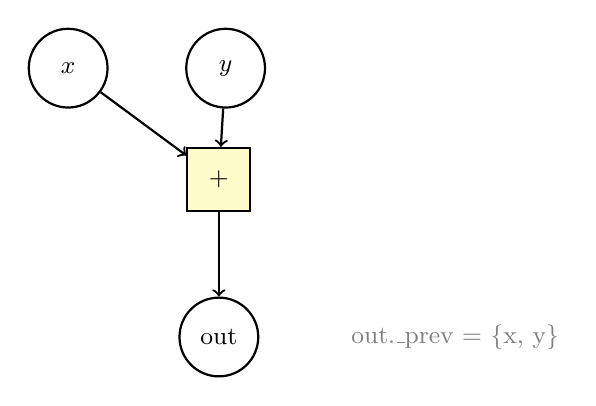
\begin{tikzpicture}[
    node distance=2cm,
    var/.style={circle, draw, thick, minimum size=1cm, font=\small},
    op/.style={rectangle, draw, thick, fill=yellow!20, minimum size=0.8cm, font=\small}
]
    \node[var] (x) {$x$};
    \node[var] (y) [right of=x] {$y$};
    \node[op] (plus) [below right of=x, xshift=0.5cm] {$+$};
    \node[var] (out) [below of=plus] {out};
    
    \draw[->, thick] (x) -- (plus);
    \draw[->, thick] (y) -- (plus);
    \draw[->, thick] (plus) -- (out);
    
    \node[right of=out, xshift=1cm, font=\small, text=gray] {out.\_prev = \{x, y\}};
\end{tikzpicture}
\caption{加法运算在内存中建立的计算图结构}
\end{figure}

\subsection{Step 3：重载乘法——记录``乘法节点''}

\begin{lstlisting}[style=teaching, language=Python]
    def __mul__(self, other):
        other = other if isinstance(other, Variable) else Variable(other)
        out = Variable(self.data * other.data, (self, other), '*')

        def _backward():
            # 对 z = x * y：dz/dx = y, dz/dy = x
            self.grad += out.grad * other.data
            other.grad += out.grad * self.data

        out._backward = _backward
        return out
\end{lstlisting}

乘法的反向规则稍复杂：$\frac{\partial(xy)}{\partial x} = y$，$\frac{\partial(xy)}{\partial y} = x$。

\textbf{关键洞察}：每一次运算都会新增一个节点，每个节点都带着``反向怎么走''的局部规则。这就是自动微分的本质——\textbf{记录计算过程 + 链式法则}。

\subsection{Step 4：backward()——从输出往回走一遍计算图}

\begin{lstlisting}[style=teaching, language=Python]
    def backward(self):
        """反向传播：拓扑排序 + 逆序执行 _backward"""
        
        topo = []       # 存拓扑序列（从叶子到输出）
        visited = set()

        def build_topo(v):
            if v not in visited:
                visited.add(v)
                for child in v._prev:
                    build_topo(child)
                topo.append(v)  # 所有前驱处理完再追加自己

        build_topo(self)  # 从输出节点开始，遍历整张计算图
        
        self.grad = np.ones_like(self.data)  # dL/dL = 1，反向传播起点
        
        for v in reversed(topo):  # 逆拓扑序：从输出到输入
            v._backward()
\end{lstlisting}

\textbf{这里在内存/函数调用上的流程是}：

\begin{enumerate}
    \item \texttt{build\_topo(self)}：从输出节点开始，递归访问 \texttt{\_prev} 指向的所有父节点。先遍历父亲，再把当前节点 \texttt{append} 到 \texttt{topo}。结果：\texttt{topo = [叶子节点, ..., 中间节点, ..., 输出节点]}
    
    \item 设置输出节点 \texttt{self.grad = 1}：数学上是 $\frac{\partial L}{\partial L} = 1$
    
    \item \texttt{for v in reversed(topo)}：从输出节点开始，按依赖顺序反向遍历。对每个节点调用 \texttt{v.\_backward()}，里面会读 \texttt{out.grad}，按链式法则更新父节点的 \texttt{grad}。
\end{enumerate}

你可以把这看成：
\begin{itemize}
    \item \texttt{build\_topo}：在内存里从 \texttt{self} 沿 \texttt{\_prev} 指针，把计算图``铺平''成一个列表
    \item \texttt{reversed(topo)}：从输出往叶子走一遍，把梯度一层层推回去
\end{itemize}

\subsection{Step 5：完整示例——生成一棵具体的计算图}

\begin{lstlisting}[style=teaching, language=Python]
# 使用示例：y = x^2 + 2x + 1
x = Variable(3.0)            # 叶子节点
y = x * x + x * 2 + 1        # 构图（每一步运算都在建计算图）
y.backward()                 # 从 y 往回传播梯度

print(f"x = {x.data}")       # 3.0
print(f"y = {y.data}")       # 16.0
print(f"dy/dx = {x.grad}")   # 8.0（理论值：2x + 2 = 8）
\end{lstlisting}

\textbf{我们详细看一下这三行代码执行时，内存中发生了什么}：

\paragraph{第一步：\texttt{x = Variable(3.0)}}

新建对象 \texttt{x}：
\begin{itemize}
    \item \texttt{x.data = 3.0}
    \item \texttt{x.grad = 0.0}
    \item \texttt{x.\_prev = $\emptyset$}（叶子节点，没有父节点）
    \item \texttt{x.\_backward = lambda: None}
\end{itemize}

此时图上只有一个孤立的点 $x$。

\paragraph{第二步：\texttt{y = x * x + x * 2 + 1}}

\textbf{关键问题}：这行代码是被谁``拆''成一步步运算的？

答案是：\textbf{Python 解释器自己拆的}。我们并没有写任何``解析器''，而是利用了 Python 的运算符重载机制。

当 Python 解释器遇到 \texttt{x * x + x * 2 + 1} 时，它按照\textbf{运算符优先级}（先乘除后加减，从左到右）依次执行：

\begin{center}
\begin{tikzpicture}[
    node distance=0.8cm,
    box/.style={draw, rounded corners, minimum width=3cm, minimum height=0.7cm, font=\small\ttfamily},
    arrow/.style={->, thick, >=stealth}
]
    % 原始表达式
    \node[box, fill=gray!10] (expr) {x * x + x * 2 + 1};
    \node[left of=expr, xshift=-2cm, font=\small] {原始表达式};

    % Step 1
    \node[box, fill=blue!10] (s1) [below=of expr] {(x * x) + x * 2 + 1};
    \node[left of=s1, xshift=-2cm, font=\small] {Step 1};
    \node[anchor=west, font=\small, text=gray] at ([xshift=1.8cm]s1.east) {调用 \texttt{x.\_\_mul\_\_(x)} $\to$ 返回 $m_1$};

    % Step 2
    \node[box, fill=blue!10] (s2) [below=of s1] {m1 + (x * 2) + 1};
    \node[left of=s2, xshift=-2cm, font=\small] {Step 2};
    \node[anchor=west, font=\small, text=gray] at ([xshift=1.8cm]s2.east) {调用 \texttt{x.\_\_mul\_\_(2)} $\to$ 返回 $m_2$};

    % Step 3
    \node[box, fill=green!10] (s3) [below=of s2] {(m1 + m2) + 1};
    \node[left of=s3, xshift=-2cm, font=\small] {Step 3};
    \node[anchor=west, font=\small, text=gray] at ([xshift=1.8cm]s3.east) {调用 \texttt{m1.\_\_add\_\_(m2)} $\to$ 返回 $s_1$};

    % Step 4
    \node[box, fill=green!10] (s4) [below=of s3] {s1 + 1};
    \node[left of=s4, xshift=-2cm, font=\small] {Step 4};
    \node[anchor=west, font=\small, text=gray] at ([xshift=1.8cm]s4.east) {调用 \texttt{s1.\_\_add\_\_(1)} $\to$ 返回 $y$};

    % 最终
    \node[box, fill=red!10] (final) [below=of s4] {y};
    \node[left of=final, xshift=-2cm, font=\small] {完成};

    % 箭头
    \draw[arrow] (expr) -- (s1);
    \draw[arrow] (s1) -- (s2);
    \draw[arrow] (s2) -- (s3);
    \draw[arrow] (s3) -- (s4);
    \draw[arrow] (s4) -- (final);
\end{tikzpicture}
\end{center}

每次调用 \texttt{\_\_mul\_\_} 或 \texttt{\_\_add\_\_} 时，我们不仅计算了数值，还\textbf{顺便}创建了一个新节点、记录了依赖关系、存下了反向传播规则。Python 解释器替我们完成了``表达式解析''的工作！

\marginnote{这就是运算符重载的威力：用户写的是普通数学表达式，背后却自动构建了完整的计算图。PyTorch、TensorFlow 都是这个原理。}

现在让我们看看每一步具体发生了什么：

\begin{enumerate}
    \item \textbf{\texttt{x * x}}：Python 调用 \texttt{x.\_\_mul\_\_(x)}，建立乘法节点 $m_1$
    \begin{itemize}
        \item $m_1$\texttt{.data} = 9.0
        \item $m_1$\texttt{.\_prev} = \{$x$\}（\texttt{set} 会去重；但闭包里对 \texttt{x.grad} 累加了两次）
        \item $m_1$\texttt{.\_backward} 存下闭包：两次累加 \texttt{x.grad += m1.grad * x.data}
    \end{itemize}
    
    \item \textbf{\texttt{x * 2}}：Python 调用 \texttt{x.\_\_mul\_\_(2)}
    \begin{itemize}
        \item 因为 \texttt{2} 不是 \texttt{Variable}，在 \texttt{\_\_mul\_\_} 内部被包装成 \texttt{Variable(2)}
        \item 建立乘法节点 $m_2$，$m_2$\texttt{.data} = 6.0，$m_2$\texttt{.\_prev} = \{$x$, const$_2$\}
    \end{itemize}
    
    \item \textbf{\texttt{m1 + m2}}：Python 调用 \texttt{m1.\_\_add\_\_(m2)}，建立加法节点 $s_1$
    \begin{itemize}
        \item $s_1$\texttt{.data} = 15.0
        \item $s_1$\texttt{.\_prev} = \{$m_1$, $m_2$\}
    \end{itemize}
    
    \item \textbf{\texttt{s1 + 1}}：Python 调用 \texttt{s1.\_\_add\_\_(1)}，\texttt{1} 被包装，建立加法节点 $y$
    \begin{itemize}
        \item $y$\texttt{.data} = 16.0
        \item $y$\texttt{.\_prev} = \{$s_1$, const$_1$\}
    \end{itemize}
\end{enumerate}

此时内存中的计算图：

\begin{figure}[h]
\centering
\begin{tikzpicture}[
    node distance=1.5cm,
    var/.style={circle, draw, thick, minimum size=0.9cm, font=\small},
    const/.style={circle, draw, dashed, minimum size=0.7cm, font=\scriptsize, text=gray},
    op/.style={rectangle, draw, thick, fill=yellow!20, minimum width=0.6cm, font=\small}
]
    % 叶子节点
    \node[var, fill=blue!10] (x) {$x$};
    \node[below of=x, yshift=0.8cm, font=\scriptsize] {3.0};
    
    % 常数节点
    \node[const] (c2) [right of=x, xshift=1cm] {2};
    \node[const] (c1) [right of=c2, xshift=2cm] {1};
    
    % 中间节点
    \node[var] (m1) [below of=x, xshift=-0.5cm, yshift=-0.5cm] {$m_1$};
    \node[below of=m1, yshift=0.8cm, font=\scriptsize] {9.0};
    
    \node[var] (m2) [below of=x, xshift=1.5cm, yshift=-0.5cm] {$m_2$};
    \node[below of=m2, yshift=0.8cm, font=\scriptsize] {6.0};
    
    \node[var] (s1) [below of=m1, xshift=1cm, yshift=-0.3cm] {$s_1$};
    \node[below of=s1, yshift=0.8cm, font=\scriptsize] {15.0};
    
    \node[var, fill=red!10] (y) [below of=s1, xshift=1cm, yshift=-0.3cm] {$y$};
    \node[below of=y, yshift=0.8cm, font=\scriptsize] {16.0};
    
    % 连线
    \draw[->, thick] (x) -- (m1);
    \draw[->, thick] (x) to[bend left=20] (m1);
    \draw[->, thick] (x) -- (m2);
    \draw[->, thick] (c2) -- (m2);
    \draw[->, thick] (m1) -- (s1);
    \draw[->, thick] (m2) -- (s1);
    \draw[->, thick] (s1) -- (y);
    \draw[->, thick] (c1) -- (y);
    
    % 标注
    \node[right of=y, xshift=1.5cm, font=\small, align=left] {
        每个节点存着：\\
        \texttt{data}（前向值）\\
        \texttt{grad}（反向值，目前全0）\\
        \texttt{\_prev}（入边）\\
        \texttt{\_backward}（局部规则）
    };
\end{tikzpicture}
\caption{执行 \texttt{y = x*x + x*2 + 1} 后内存中的计算图}
\end{figure}

\paragraph{第三步：\texttt{y.backward()}}

\begin{enumerate}
    \item \texttt{build\_topo(y)} 得到拓扑序列（满足``父在前，子在后''）：
$    \texttt{topo} = [x, \text{const}_2, m_2, m_1, s_1, \text{const}_1, y]$
    
    \item 设置输出节点的梯度（反向传播起点）：
$    \frac{\partial y}{\partial y} = 1 \quad \Rightarrow \quad \texttt{y.grad} = 1
$    
    
    \item 逆序遍历 \texttt{topo}，执行每个节点的 \texttt{\_backward()}：
\end{enumerate}

\begin{center}
\renewcommand{\arraystretch}{1.6}
\begin{tabular}{c|l|l}
\toprule
\textbf{节点} & \textbf{执行的反向规则} & \textbf{梯度更新} \\
\midrule
$y$ & $y = s_1 + 1$，加法反传 & $\displaystyle \frac{\partial y}{\partial s_1} = 1 \;\Rightarrow\; s_1.\text{grad} \mathrel{+}= 1$ \\[3pt]
\midrule
$s_1$ & $s_1 = m_1 + m_2$，加法反传 & $\displaystyle \frac{\partial y}{\partial m_1} = \frac{\partial y}{\partial s_1} \cdot 1 = 1 \;\Rightarrow\; m_1.\text{grad} \mathrel{+}= 1$ \\
 & & $\displaystyle \frac{\partial y}{\partial m_2} = \frac{\partial y}{\partial s_1} \cdot 1 = 1 \;\Rightarrow\; m_2.\text{grad} \mathrel{+}= 1$ \\[3pt]
\midrule
$m_1$ & $m_1 = x \cdot x$，乘法反传 & $\displaystyle \frac{\partial y}{\partial x} \mathrel{+}= \frac{\partial y}{\partial m_1} \cdot x = 1 \times 3 = 3$ \\
 & （$x$出现两次，累加两次） & $\displaystyle \frac{\partial y}{\partial x} \mathrel{+}= \frac{\partial y}{\partial m_1} \cdot x = 1 \times 3 = 3$ \\
 & & $\Rightarrow\; x.\text{grad} = 0 + 3 + 3 = 6$ \\[3pt]
\midrule
$m_2$ & $m_2 = x \cdot 2$，乘法反传 & $\displaystyle \frac{\partial y}{\partial x} \mathrel{+}= \frac{\partial y}{\partial m_2} \cdot 2 = 1 \times 2 = 2$ \\
 & & $\Rightarrow\; x.\text{grad} = 6 + 2 = 8$ \\[3pt]
\midrule
$x$ & 叶子节点，无 \texttt{\_prev} & 反向传播结束 \\
\bottomrule
\end{tabular}
\end{center}

\vspace{0.3cm}
\noindent\textbf{最终结果}：
\begin{equation*}
x.\text{grad} = 8 = 2x + 2 \big|_{x=3} = \frac{dy}{dx}
\end{equation*}

\marginnote{PyTorch的\texttt{autograd}和这个简化版本原理完全相同，只是添加了：GPU支持、更多运算符、内存优化、支持高阶导数等工程细节。理解了这50行代码，你就理解了现代深度学习框架的核心。}

\begin{physicalmeaning}
这个极简引擎揭示了自动微分的本质：
\begin{itemize}
    \item \textbf{前向传播}：执行计算的同时，在内存中搭建一棵``函数树''
    \item \textbf{反向传播}：从树根（输出）往叶子走一遍，用链式法则把梯度一层层推回去
    \item \textbf{每个节点的 \texttt{\_backward}}：就是伴随方程的``局部版本''
\end{itemize}

这正是拉格朗日方法的计算机实现：每个节点只需要知道自己的``邻居''，不需要了解整张图的结构。
\end{physicalmeaning}
\tryit{给 \texttt{Variable} 加上 \texttt{\_\_pow\_\_} 和 \texttt{exp()}，对 $y = \exp(x^2)$ 调用 \texttt{backward()}，再用中心差分 $[y(x+h) - y(x-h)]/2h$ 核对 \texttt{x.grad}。这是习题4的热身。}


\section{梯度下降与优化器}
有了梯度，下一步就是用它来更新参数。这一节介绍深度学习中常用的优化方法。

回顾本章开头：训练就是 $\min_\theta L(\theta)$——一个关于参数 $\theta$ 的\textbf{无约束}优化问题（约束已经被伴随变量"消化"进梯度里了）。最直接的办法是梯度下降。它看起来很简单，但在真正训练一个大型神经网络时会遇到几个实际困难：
\begin{itemize}
    \item 数据量很大，不可能每次都计算全部样本；
    \item 损失地形很复杂，可能像峡谷一样又弯又深；
    \item 不同方向的梯度大小差异巨大，导致震荡或停滞；
    \item 学习率太大不行、太小也不行。
\end{itemize}

接下来，我们将看到 SGD、动量法和 Adam 等方法是如何一步步解决这些问题的。


\subsection{vanilla 梯度下降}

最基本的更新规则：
\begin{equation}
\theta^{(t+1)} = \theta^{(t)} - \eta \nabla_\theta L(\theta^{(t)})
\end{equation}

其中 $\eta > 0$ 是\textbf{学习率}（learning rate），控制每一步走多远。

\begin{figure}[h]
\centering
\begin{tikzpicture}[scale=1.2]
    % 等高线
    \foreach \r in {0.5, 1, 1.5, 2, 2.5} {
        \draw[gray!50] (0,0) ellipse ({\r} and {\r*0.6});
    }
    
    % 梯度下降路径
    \coordinate (p0) at (2.2, 0.8);
    \coordinate (p1) at (1.5, 0.4);
    \coordinate (p2) at (0.9, 0.15);
    \coordinate (p3) at (0.4, 0.05);
    \coordinate (p4) at (0.1, 0.01);
    
    \fill[blue] (p0) circle (2pt) node[above right] {$\theta^{(0)}$};
    \fill[blue] (p1) circle (2pt);
    \fill[blue] (p2) circle (2pt);
    \fill[blue] (p3) circle (2pt);
    \fill[red] (p4) circle (2pt) node[below] {$\theta^*$};
    
    \draw[->, thick, blue] (p0) -- (p1);
    \draw[->, thick, blue] (p1) -- (p2);
    \draw[->, thick, blue] (p2) -- (p3);
    \draw[->, thick, blue] (p3) -- (p4);
    
    % 标注
    \node at (0, -2) {损失函数的等高线};
\end{tikzpicture}
\caption{梯度下降：沿着负梯度方向，一步步走向最小值点}
\end{figure}

\textbf{学习率的选择}是一门艺术：
\begin{itemize}
    \item $\eta$ 太大：可能跳过最优点，甚至发散
    \item $\eta$ 太小：收敛太慢，训练时间过长
\end{itemize}

\subsection{随机梯度下降（SGD）}

\marginnote{\textbf{SGD的起源}：随机梯度下降由Robbins和Monro在1951年提出（``A Stochastic Approximation Method''），最初用于统计估计问题。半个多世纪后，它成为训练深度神经网络的标准方法，每天在全球数百万GPU上运行。}

当数据集很大时，计算全部样本的梯度太慢。\textbf{随机梯度下降}的想法是：每次只用一小批样本（mini-batch）来估计梯度。

\begin{keyformula}[title=Mini-batch SGD]
每次迭代：
\begin{enumerate}
    \item 从训练集中随机抽取一个小批量 $\mathcal{B} = \{(x^{(i)}, y^{(i)})\}_{i=1}^B$
    \item 计算这个批量上的平均梯度：
    \begin{equation}
    g = \frac{1}{B} \sum_{i \in \mathcal{B}} \nabla_\theta \ell(f(x^{(i)}; \theta), y^{(i)})
    \end{equation}
    \item 更新参数：$\theta \leftarrow \theta - \eta \cdot g$
\end{enumerate}
\end{keyformula}

\marginnote{为什么随机梯度也能收敛？因为 $\E[g] = \nabla_\theta L$，即小批量梯度是真实梯度的无偏估计。虽然每一步有噪声，但平均方向是对的。}

典型的批量大小 $B$ 是 32、64、128 或 256。

\subsection{动量法（Momentum）}

\marginnote{\textbf{动量法的历史}：动量方法由苏联数学家Boris Polyak于1964年提出（``Some methods of speeding up the convergence of iteration methods''）。这个简单而优雅的想法——给梯度加上``惯性''——至今仍是训练大型视觉模型（如ResNet、ViT）的首选方法。}

vanilla SGD 的问题：在``峡谷''地形中会来回震荡，收敛很慢。

\textbf{动量法}的想法：引入``惯性''，让更新方向更平滑。

\begin{keyformula}[title=SGD with Momentum]
\begin{align}
v^{(t+1)} &= \beta \cdot v^{(t)} + \nabla_\theta L(\theta^{(t)}) \\
\theta^{(t+1)} &= \theta^{(t)} - \eta \cdot v^{(t+1)}
\end{align}

其中 $v$ 是\textbf{速度}（velocity），$\beta \in [0, 1)$ 是动量系数（通常取 0.9）。
\end{keyformula}

\begin{physicalmeaning}
可以把优化过程想象成一个小球在损失曲面上滚动：
\begin{itemize}
    \item 没有动量：小球每一步只看当前坡度，容易来回震荡
    \item 有动量：小球有惯性，能``冲过''小坑，沿着主方向加速
\end{itemize}
\end{physicalmeaning}
\review{第4章}{"小球在损失曲面上滚"不只是比喻：把动量法写成连续时间，就是带阻尼的牛顿方程 $\ddot{\theta} + \gamma\dot{\theta} = -\nabla L(\theta)$——第4章的力学，势能就是损失函数，动量系数 $\beta$ 决定阻尼大小。}

\subsection{Adam：自适应学习率}

\marginnote{\textbf{Adam的诞生}：Adam由阿姆斯特丹大学的Diederik Kingma和多伦多大学的Jimmy Ba于2014年提出，发表于ICLR 2015。它巧妙地结合了动量法和RMSprop（Hinton课程中提出）的思想。论文引用超过20万次，Adam成为深度学习中最广泛使用的优化器之一，尤其在NLP和Transformer训练中几乎是标配。}

不同参数可能需要不同的学习率。\textbf{Adam}（Adaptive Moment Estimation）自动为每个参数调整学习率。

\begin{keyformula}[title=Adam 优化器]
\begin{align}
m^{(t+1)} &= \beta_1 m^{(t)} + (1 - \beta_1) g^{(t)} \quad \text{（一阶矩估计，类似动量）} \\
v^{(t+1)} &= \beta_2 v^{(t)} + (1 - \beta_2) (g^{(t)})^2 \quad \text{（二阶矩估计，梯度平方的滑动平均）} \\[5pt]
\hat{m} &= \frac{m^{(t+1)}}{1 - \beta_1^{t+1}}, \quad \hat{v} = \frac{v^{(t+1)}}{1 - \beta_2^{t+1}} \quad \text{（偏差修正）} \\[5pt]
\theta^{(t+1)} &= \theta^{(t)} - \eta \cdot \frac{\hat{m}}{\sqrt{\hat{v}} + \epsilon}
\end{align}

默认超参数：$\beta_1 = 0.9$，$\beta_2 = 0.999$，$\epsilon = 10^{-8}$，$\eta = 0.001$。
\end{keyformula}

\textbf{Adam 的直觉}：
\begin{itemize}
    \item $m$：梯度的滑动平均，提供动量效果
    \item $v$：梯度平方的滑动平均，估计每个参数的``典型梯度大小''
    \item 更新量 $\propto \frac{m}{\sqrt{v}}$：梯度大的方向步子小，梯度小的方向步子大
\end{itemize}

\subsection{优化器对比}

\begin{center}
\renewcommand{\arraystretch}{1.4}
\begin{tabular}{l|c|c|l}
\toprule
\textbf{优化器} & \textbf{自适应学习率} & \textbf{动量} & \textbf{适用场景} \\
\midrule
SGD & 否 & 否 & 简单问题，需要仔细调参 \\
SGD + Momentum & 否 & 是 & 大多数视觉任务 \\
Adam & 是 & 是 & NLP、快速原型、默认选择 \\
AdamW & 是 & 是 & Adam + 权重衰减，Transformer标配 \\
\bottomrule
\end{tabular}
\end{center}

\marginnote{实践中的经验：Adam 收敛快但泛化可能略差；SGD+Momentum 需要更多调参但最终效果常常更好。很多顶级模型用 SGD+Momentum 训练。}

\subsection{完整训练循环}

把前面所有内容串起来，一个完整的神经网络训练循环是这样的：

\begin{lstlisting}[style=teaching, language=Python]
# 伪代码：完整的训练循环
def train(model, data_loader, optimizer, num_epochs):
    for epoch in range(num_epochs):
        for batch_x, batch_y in data_loader:
            # 1. 前向传播：计算预测值和损失
            predictions = model.forward(batch_x)
            loss = compute_loss(predictions, batch_y)
            
            # 2. 反向传播：计算所有参数的梯度
            loss.backward()  # 自动微分！
            
            # 3. 参数更新：用优化器更新参数
            optimizer.step()  # theta = theta - lr * grad
            
            # 4. 清零梯度：为下一次迭代做准备
            optimizer.zero_grad()
        
        print(f"Epoch {epoch}: loss = {loss.item()}")
\end{lstlisting}

\begin{figure}[h]
\centering
\begin{tikzpicture}[
    box/.style={draw, rounded corners, minimum width=2.8cm, minimum height=1cm, font=\small, align=center},
    arrow/.style={->, thick, >=stealth}
]
    \node[box, fill=blue!15] (forward) at (0, 0) {前向传播\\$L = \ell(f(x; \theta), y)$};
    \node[box, fill=red!15] (backward) at (5, 0) {反向传播\\$\nabla_\theta L$};
    \node[box, fill=green!15] (update) at (10, 0) {参数更新\\$\theta \leftarrow \theta - \eta g$};
    
    \draw[arrow] (forward) -- node[above, font=\scriptsize] {计算损失} (backward);
    \draw[arrow] (backward) -- node[above, font=\scriptsize] {计算梯度} (update);
    \draw[arrow, dashed] (update.south) -- ++(0, -0.8) -| node[below, pos=0.25, font=\scriptsize] {下一个 batch} (forward.south);
\end{tikzpicture}
\caption{训练循环的三个核心步骤}
\end{figure}

这就是深度学习训练的完整流程：
\begin{enumerate}
    \item \textbf{前向传播}：用当前参数计算预测和损失
    \item \textbf{反向传播}：用伴随方程（自动微分）计算梯度
    \item \textbf{参数更新}：用优化器沿负梯度方向更新参数
    \item 重复以上步骤，直到损失收敛
\end{enumerate}

% ------------------------------------------------------------------------------------
% 代码演示结果
\begin{figure}[htbp]
\centering
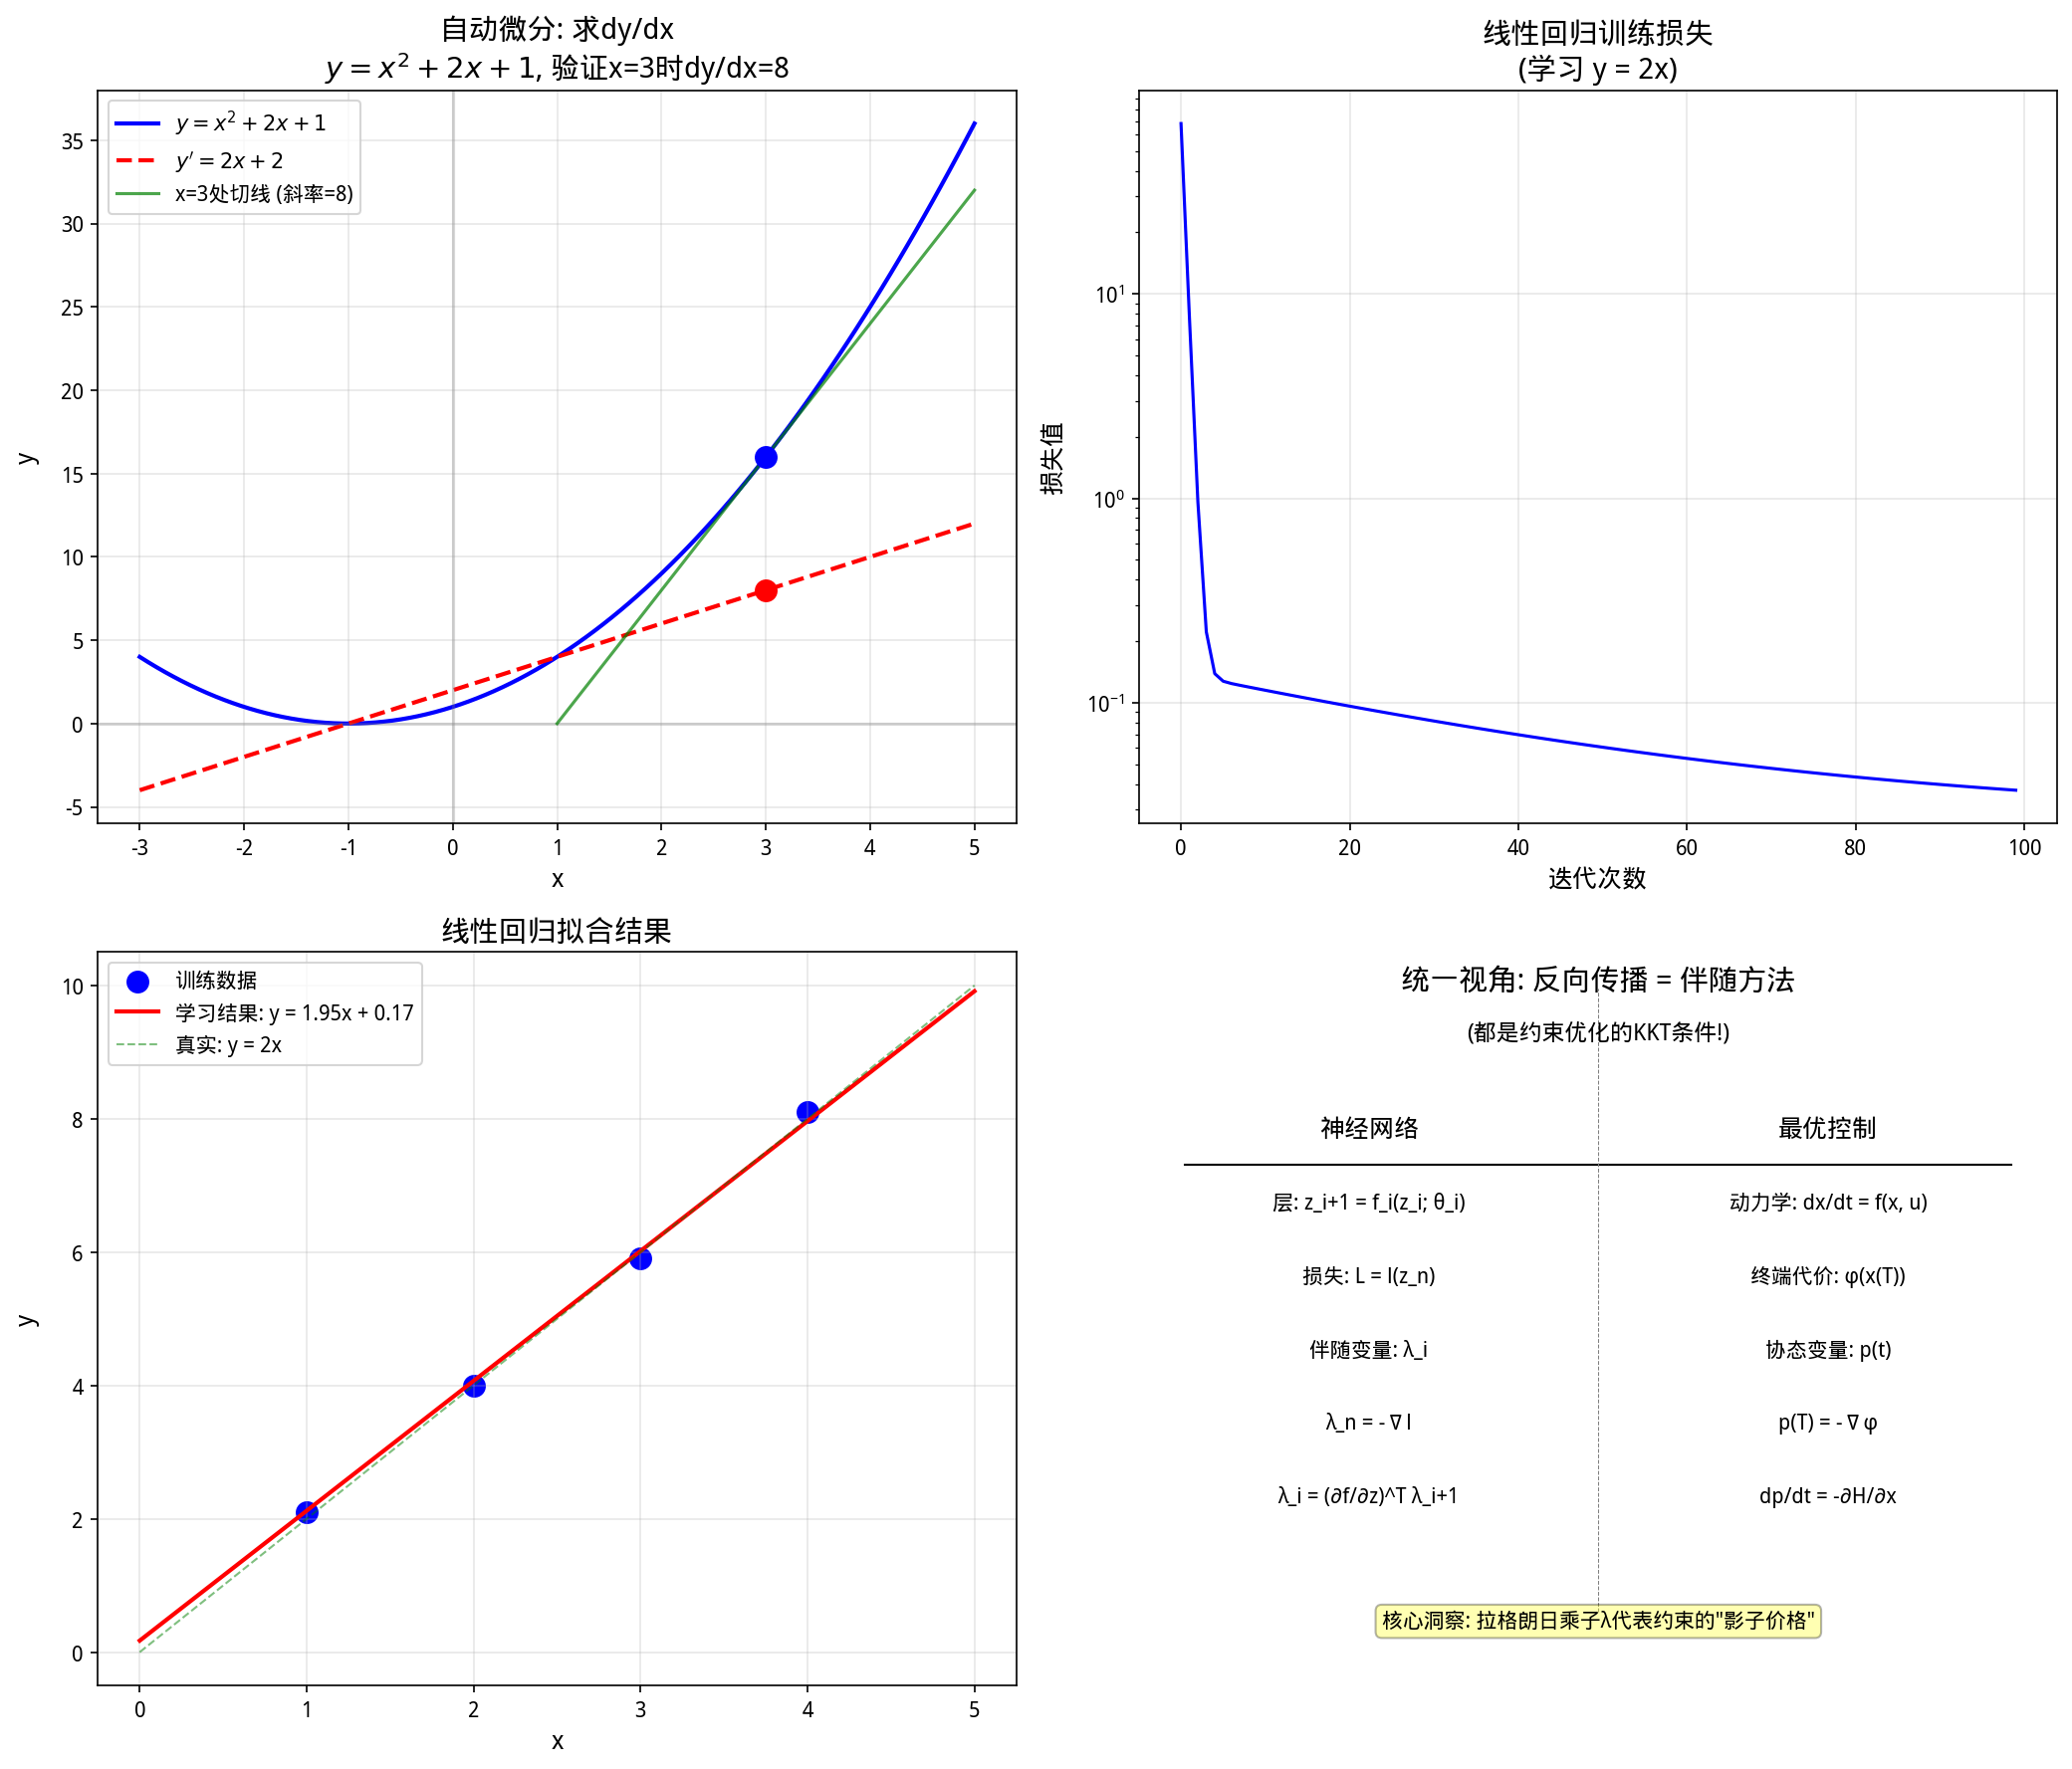
\includegraphics[width=0.95\textwidth]{figs_chap09/chap09_fig1.png}
\caption{自动微分与反向传播演示。（1）自动微分验证：本章例子 $y = x^2 + 2x + 1$，自动微分给出 $x = 3$ 处的切线斜率 $dy/dx = 8$，与手算一致；（2）用自动微分引擎训练线性回归 $y = 2x$ 的损失曲线；（3）拟合结果；（4）统一视角：神经网络的伴随变量 $\lambda_i$ 与最优控制的协态变量 $p(t)$ 逐项对应——都是约束优化的 KKT 条件。}
\label{fig:chap09_autograd}
\end{figure}

% ------------------------------------------------------------------------------------
\section{本章小结}

本章建立了深度学习与约束优化之间的桥梁：

\begin{enumerate}
    \item \textbf{神经网络}是一类参数化的复合函数，通过堆叠简单的线性变换和非线性激活来逼近复杂映射。
    
    \item \textbf{训练}是一个优化问题：最小化损失函数，找到最优参数。
    
    \item \textbf{计算图视角}：把复合函数展开为中间变量，每层变成一个等式约束。
    
    \item \textbf{拉格朗日函数}：引入乘子 $\lambda_i$，KKT条件给出伴随方程——这就是反向传播。
    
    \item \textbf{$\lambda_i$ 的意义}：第 $i$ 层输出对最终损失的敏感度，等价于``影子价格''。
    
    \item \textbf{统一框架}：反向传播 = 离散伴随方程 = 最优控制的数值版本。
\end{enumerate}

\begin{unification}[title=统一视角：伴随方法的三种面孔]
\begin{center}
\begin{tabular}{lll}
\toprule
\textbf{领域} & \textbf{正向过程} & \textbf{反向过程（伴随）} \\
\midrule
神经网络 & 前向传播 & 反向传播 \\
最优控制 & 状态方程 & 协态方程 \\
有限元/PDE & 求解原问题 & 敏感度分析 \\
\bottomrule
\end{tabular}
\end{center}
\end{unification}

\begin{physicalmeaning}
\textbf{$\lambda$ 在本章的意义}：$\lambda_i$ 是第 $i$ 层等式约束的影子价格——把第 $i$ 层的输出 $z_i$ 悄悄改动 $\epsilon$，最终损失变化 $-\lambda_i^\top \epsilon$。深度学习管 $\delta_i = -\lambda_i$ 叫"误差信号"，控制论管它叫"协态"，第1章管它叫"影子价格"——三个名字，一个东西。
\begin{itemize}
    \item 第8章：把"层 $i$"换成"时刻 $k$"、把参数 $\theta_i$ 换成控制 $u_k$，本章的伴随方程逐字变回第8章的离散伴随方程。
    \item 第10章：把损失换成"未来累计奖励"（符号因此翻转，$\lambda = +\partial J/\partial s$），把网络深度推到无穷，$\lambda$ 变成值函数的梯度，伴随方程变成贝尔曼方程。
    \item 第13章：把自动微分反过来用——不是对参数求导，而是对输入坐标 $(x, t)$ 求导，就能把偏微分方程本身写进损失函数（PINN）。
\end{itemize}
\end{physicalmeaning}

% ------------------------------------------------------------------------------------
\section{习题}

\paragraph{计算题}
\begin{enumerate}
    \item 考虑单层网络 $y = \sigma(Wx + b)$，损失 $L = \frac{1}{2}\|y - t\|^2$。
    \begin{enumerate}
        \item 写出拉格朗日函数。
        \item 推导 $\nabla_W L$ 和 $\nabla_b L$ 的表达式。
        \item 若 $\sigma(x) = \max(0, x)$（ReLU），写出梯度的具体形式。
    \end{enumerate}
    
    \item 对于softmax输出 $p_i = \frac{e^{z_i}}{\sum_j e^{z_j}}$ 和交叉熵损失 $L = -\sum_i y_i \log p_i$，证明 $\frac{\partial L}{\partial z_i} = p_i - y_i$。
    
    \item 考虑带skip connection的残差块：$z_{i+1} = z_i + f_i(z_i; \theta_i)$。推导它的伴随方程。
\end{enumerate}

\paragraph{编程题}
\begin{enumerate}
    \setcounter{enumi}{3}
    \item 扩展本章的自动微分引擎，添加以下运算：
    \begin{itemize}
        \item 矩阵乘法 $Y = XW$
        \item ReLU激活函数
        \item 交叉熵损失
    \end{itemize}
    
    \item 用你的引擎训练一个两层神经网络，在MNIST数据集的一个子集上进行手写数字分类。对比PyTorch的结果。
\end{enumerate}

\paragraph{思考题}
\begin{enumerate}
    \setcounter{enumi}{5}
    \item ``反向传播就是链式法则的应用''——这个常见说法有什么不准确之处？
    
    \item 为什么说反向传播是``空间换时间''的算法？它需要存储什么？
    
    \item 如果我们想计算二阶导数（Hessian矩阵），能否用类似的方法？这与``Hessian-free''优化有什么关系？
\end{enumerate}

\section*{扩展阅读：矩阵求导的规则与设计哲学}
\addcontentsline{toc}{section}{扩展阅读：矩阵求导}

在推导反向传播时，我们不可避免地要对矩阵、向量求导。这里系统介绍矩阵微积分的规则，更重要的是，解释\textbf{为什么}规则要这样设计。

\subsection*{核心问题：导数的``形状''应该是什么？}

考虑一个简单的问题：$y = Wx$，其中 $W \in \R^{m \times n}$，$x \in \R^n$，$y \in \R^m$。

问：$\frac{\partial y}{\partial x}$ 的形状应该是什么？

\textbf{直觉上}，$y$ 有 $m$ 个分量，$x$ 有 $n$ 个分量，所以导数应该有 $m \times n$ 个元素。但这 $m \times n$ 个元素应该排成什么形状？$m \times n$ 还是 $n \times m$？

这不是一个有唯一正确答案的问题——它是一个\textbf{约定}问题。不同的约定导致不同的``布局''（layout）。

\subsection*{两种布局约定}

\begin{definition}[雅可比矩阵的两种布局]
设 $f: \R^n \to \R^m$，即 $y = f(x)$，其中 $x \in \R^n$，$y \in \R^m$。

\textbf{分子布局}（Numerator Layout）：
\begin{equation}
\frac{\partial y}{\partial x} = \begin{pmatrix}
\frac{\partial y_1}{\partial x_1} & \frac{\partial y_1}{\partial x_2} & \cdots & \frac{\partial y_1}{\partial x_n} \\
\frac{\partial y_2}{\partial x_1} & \frac{\partial y_2}{\partial x_2} & \cdots & \frac{\partial y_2}{\partial x_n} \\
\vdots & \vdots & \ddots & \vdots \\
\frac{\partial y_m}{\partial x_1} & \frac{\partial y_m}{\partial x_2} & \cdots & \frac{\partial y_m}{\partial x_n}
\end{pmatrix} \in \R^{m \times n}
\end{equation}
第 $i$ 行第 $j$ 列是 $\frac{\partial y_i}{\partial x_j}$。行数跟分子走，列数跟分母走。

\textbf{分母布局}（Denominator Layout）：
\begin{equation}
\frac{\partial y}{\partial x} = \begin{pmatrix}
\frac{\partial y_1}{\partial x_1} & \frac{\partial y_2}{\partial x_1} & \cdots & \frac{\partial y_m}{\partial x_1} \\
\frac{\partial y_1}{\partial x_2} & \frac{\partial y_2}{\partial x_2} & \cdots & \frac{\partial y_m}{\partial x_2} \\
\vdots & \vdots & \ddots & \vdots \\
\frac{\partial y_1}{\partial x_n} & \frac{\partial y_2}{\partial x_n} & \cdots & \frac{\partial y_m}{\partial x_n}
\end{pmatrix} \in \R^{n \times m}
\end{equation}
就是分子布局的转置。行数跟分母走，列数跟分子走。
\end{definition}

\textbf{两种布局互为转置}，没有对错之分，只有方便与否。

\subsection*{为什么深度学习偏好分母布局？}

深度学习中，我们最关心的是\textbf{标量对向量的导数}：损失 $L$ 对参数 $\theta$ 的梯度。

设 $L \in \R$（标量），$\theta \in \R^n$（向量）。

\begin{itemize}
    \item \textbf{分子布局}：$\frac{\partial L}{\partial \theta} \in \R^{1 \times n}$（行向量）
    \item \textbf{分母布局}：$\frac{\partial L}{\partial \theta} \in \R^{n \times 1}$（列向量）
\end{itemize}

分母布局的好处是：\textbf{梯度和参数形状相同}。这样梯度下降可以直接写成：
\begin{equation}
\theta^{(t+1)} = \theta^{(t)} - \eta \nabla_\theta L
\end{equation}
不需要转置。PyTorch、TensorFlow 都采用这个约定。

\marginnote{\footnotesize
在深度学习框架里（PyTorch、TensorFlow、JAX），
参数 \texttt{w} 本身就是一个 \textbf{n×1 的张量}。
如果梯度也是 n×1，就可以直接做：

\texttt{w -= lr * w.grad}

而不用写
\texttt{w -= lr * w.grad.T}

越少转置，越少 bug。
}


\subsubsection*{一个最简单的例子（为什么分母布局更顺手？）}

深度学习中，最常见的梯度是 \textbf{标量损失 $L$ 对向量参数 $\theta$ 的导数}。

\[
L \in \mathbb{R}, \qquad \theta \in \mathbb{R}^n.
\]

两种常见定义是：

\begin{itemize}
    \item \textbf{分子布局（numerator layout）}：$\displaystyle \frac{\partial L}{\partial \theta} \in \mathbb{R}^{1 \times n}$（行向量）
    \item \textbf{分母布局（denominator layout）}：$\displaystyle \nabla_\theta L = \frac{\partial L}{\partial \theta} \in \mathbb{R}^{n \times 1}$（列向量）
\end{itemize}

深度学习框架（PyTorch / TensorFlow）统一采用分母布局，因为它使得梯度和参数形状一致，更新规则非常自然。

下面通过一个能够\textbf{直接代入数字手算}的例子来说明。

\paragraph{例子：最简单的线性模型}

设参数和输入为：

\[
x=\begin{pmatrix}2 \\ 3\end{pmatrix},\qquad 
w=\begin{pmatrix}1 \\ -1\end{pmatrix},\qquad 
t=4.
\]

模型输出：

\[
y = w^\top x = 1\cdot 2 + (-1)\cdot 3 = -1.
\]

平方误差损失：

\[
L=\frac12 (y - t)^2 = \frac12(-5)^2 = 12.5.
\]

\paragraph{计算梯度}

对于线性模型，损失对参数的梯度是：

\[
\nabla_w L = (y - t)\, x.
\]

代入数值：

\[
y - t = -1 - 4 = -5,
\qquad
x = \begin{pmatrix}2 \\ 3\end{pmatrix}.
\]

因此：

\[
\nabla_w L
= -5
\begin{pmatrix}2 \\ 3\end{pmatrix}
=
\begin{pmatrix}-10 \\ -15\end{pmatrix}.
\]

注意这是一个 \textbf{列向量}，与 $w$ 的形状完全一致。

\paragraph{梯度下降更新(手算)}

设学习率 $\eta=0.1$：

\[
w_{\text{new}}
= w - \eta \nabla_w L
=
\begin{pmatrix}1 \\ -1\end{pmatrix}
- 0.1
\begin{pmatrix}-10 \\ -15\end{pmatrix}
=
\begin{pmatrix}2 \\ 0.5\end{pmatrix}.
\]

完全不需要写转置！

\paragraph{如果用分子布局会怎样？}

分子布局得到的是行向量：

\[
\frac{\partial L}{\partial w} = [-10\ -15].
\]

更新必须写成：

\[
w_{\text{new}} = w - \eta \left( \frac{\partial L}{\partial w} \right)^{\top},
\]

否则维度不匹配（行向量 vs. 列向量）。

\bigskip
\begin{tcolorbox}[title=结论, colback=yellow!10!white]
深度学习采用分母布局（列向量梯度），因为它使得：

\[
\boxed{ \text{梯度和参数形状一致，更新公式无需转置，最自然。} }
\]

\end{tcolorbox}




\subsection*{标量对向量求导}

这是最基础的情况。设 $f: \R^n \to \R$，即 $y = f(x)$ 是标量。

\begin{keyformula}[title=标量对向量的梯度]
\begin{equation}
\nabla_x f = \frac{\partial f}{\partial x} = \begin{pmatrix}
\frac{\partial f}{\partial x_1} \\
\frac{\partial f}{\partial x_2} \\
\vdots \\
\frac{\partial f}{\partial x_n}
\end{pmatrix} \in \R^n
\end{equation}
（分母布局：梯度是列向量，与 $x$ 形状相同）
\end{keyformula}

\textbf{常用公式}：
\begin{align}
\nabla_x (a^\top x) &= a \\
\nabla_x (x^\top A x) &= (A + A^\top) x \\
\nabla_x \|x\|^2 &= 2x \\
\nabla_x \|Ax - b\|^2 &= 2A^\top(Ax - b)
\end{align}

\subsection*{标量对矩阵求导}

设 $f: \R^{m \times n} \to \R$，即 $y = f(X)$ 是标量，$X$ 是矩阵。

\begin{keyformula}[title=标量对矩阵的梯度]
\begin{equation}
\nabla_X f = \frac{\partial f}{\partial X} = \begin{pmatrix}
\frac{\partial f}{\partial X_{11}} & \frac{\partial f}{\partial X_{12}} & \cdots \\
\frac{\partial f}{\partial X_{21}} & \frac{\partial f}{\partial X_{22}} & \cdots \\
\vdots & \vdots & \ddots
\end{pmatrix} \in \R^{m \times n}
\end{equation}
梯度矩阵与 $X$ 形状相同，第 $(i,j)$ 元素是 $\frac{\partial f}{\partial X_{ij}}$。
\end{keyformula}

\textbf{常用公式}：
\begin{align}
\nabla_X \tr(AX) &= A^\top \\
\nabla_X \tr(X^\top A) &= A \\
\nabla_X \tr(AXB) &= A^\top B^\top \\
\nabla_X \tr(X^\top AX) &= (A + A^\top)X \\
\nabla_X (a^\top X b) &= ab^\top
\end{align}

\marginnote{这些公式看起来复杂，但都可以通过``展开成分量，求导，再组装回去''的方法推导。关键是保持布局一致。}

\subsection*{向量对向量求导（雅可比矩阵）}

设 $f: \R^n \to \R^m$，即 $y = f(x)$，其中 $y \in \R^m$，$x \in \R^n$。

\begin{keyformula}[title=雅可比矩阵]
分子布局下：
\begin{equation}
J = \frac{\partial y}{\partial x} = \begin{pmatrix}
\frac{\partial y_1}{\partial x_1} & \cdots & \frac{\partial y_1}{\partial x_n} \\
\vdots & \ddots & \vdots \\
\frac{\partial y_m}{\partial x_1} & \cdots & \frac{\partial y_m}{\partial x_n}
\end{pmatrix} \in \R^{m \times n}
\end{equation}
第 $i$ 行是 $\nabla_{x} y_i$ 的转置。
\end{keyformula}

\textbf{常用公式}：
\begin{align}
\frac{\partial (Ax)}{\partial x} &= A \quad \text{（$A$ 是常矩阵）} \\
\frac{\partial (Ax)}{\partial A} &= ? \quad \text{（这需要更复杂的记号，见下文）}
\end{align}

\subsection*{神经网络中的关键公式}

在反向传播中，我们最常遇到的是以下几种情况：

\textbf{情况1}：$z = Wx + b$，求 $\frac{\partial L}{\partial W}$

设 $L$ 是标量损失，$\delta = \frac{\partial L}{\partial z}$ 已知（从后面传回来的梯度）。

\begin{equation}
\boxed{\frac{\partial L}{\partial W} = \delta \, x^\top}
\end{equation}

\textbf{推导}：用链式法则，$L$ 通过 $z$ 依赖于 $W$。
\begin{equation}
\frac{\partial L}{\partial W_{ij}} = \sum_k \frac{\partial L}{\partial z_k} \frac{\partial z_k}{\partial W_{ij}} = \frac{\partial L}{\partial z_i} \cdot x_j = \delta_i x_j
\end{equation}
组装成矩阵形式就是 $\delta x^\top$。

\textbf{情况2}：$z = Wx$，求 $\frac{\partial L}{\partial x}$（传给上一层的梯度）

\begin{equation}
\boxed{\frac{\partial L}{\partial x} = W^\top \delta}
\end{equation}

\textbf{推导}：
\begin{equation}
\frac{\partial L}{\partial x_j} = \sum_k \frac{\partial L}{\partial z_k} \frac{\partial z_k}{\partial x_j} = \sum_k \delta_k W_{kj} = (W^\top \delta)_j
\end{equation}

\textbf{情况3}：$z = \sigma(a)$（逐元素激活），求 $\frac{\partial L}{\partial a}$

\begin{equation}
\boxed{\frac{\partial L}{\partial a} = \delta \odot \sigma'(a)}
\end{equation}

其中 $\odot$ 是逐元素乘法（Hadamard积），$\sigma'(a)$ 是激活函数的导数逐元素作用于 $a$。

\subsection*{为什么转置会出现？}

很多初学者困惑：为什么 $\frac{\partial L}{\partial x} = W^\top \delta$ 要有转置？

\textbf{直觉解释}：前向传播时，$W$ 把 $n$ 维空间映射到 $m$ 维空间。反向传播时，梯度要从 $m$ 维空间``映射回'' $n$ 维空间。这个``反向映射''就是 $W^\top$。

\textbf{更深的理解}：$W^\top$ 是 $W$ 的\textbf{伴随算子}（adjoint）。在内积空间中，线性算子 $A$ 的伴随 $A^*$ 满足 $\langle Ax, y \rangle = \langle x, A^* y \rangle$。对于实矩阵，伴随就是转置。

这解释了为什么伴随方程（反向传播）中到处是转置——它们在数学上是前向算子的伴随。

\subsection*{记忆技巧：维度分析}

当你不确定某个公式时，\textbf{维度分析}是最可靠的检验：

\begin{itemize}
    \item $W \in \R^{m \times n}$，$x \in \R^n$，则 $Wx \in \R^m$ ✓
    \item $\delta \in \R^m$（与 $z$ 同形状），$x \in \R^n$
    \item $\frac{\partial L}{\partial W}$ 应与 $W$ 同形状，即 $\R^{m \times n}$
    \item $\delta x^\top \in \R^{m \times 1} \cdot \R^{1 \times n} = \R^{m \times n}$ ✓
\end{itemize}

\begin{insightbox}[title=实用建议]
\begin{enumerate}
    \item \textbf{坚持一种布局}：推荐分母布局（梯度与变量同形状）。
    \item \textbf{标量是安全的}：遇到复杂情况，先把 $L$ 写成标量形式，对每个分量求导，再组装。
    \item \textbf{维度检验}：每一步都检查维度是否匹配。
    \item \textbf{用迹的技巧}：$a^\top X b = \tr(ab^\top X^\top) = \tr(b a^\top X)$，迹对矩阵求导有简洁公式。
\end{enumerate}
\end{insightbox}

\subsection*{与拉格朗日方法的联系}

回到本章的主题：为什么拉格朗日方法能避免矩阵求导的混乱？

关键在于：\textbf{拉格朗日函数 $\mathcal{L}$ 是标量}。

当我们写：
\begin{equation}
\mathcal{L} = L(z_n) + \sum_i \lambda_i^\top (z_i - f_i(z_{i-1}; W_i))
\end{equation}

每一项都是标量（$\lambda_i^\top (\cdots)$ 是向量内积，结果是标量）。对标量求导：
\begin{itemize}
    \item 对向量求导 → 得到同形状的向量
    \item 对矩阵求导 → 得到同形状的矩阵
\end{itemize}

不需要处理雅可比矩阵、三阶张量这些复杂对象。转置符号也会从标量求导的规则中\textbf{自动出现}，而不需要我们去猜。

这就是拉格朗日方法的优雅之处：它把高维的矩阵微积分问题，降维成了一系列标量微积分问题。


\section*{扩展阅读：Python 如何理解 \texttt{x * x + x * 2 + 1}？}
\addcontentsline{toc}{section}{扩展阅读：Python表达式求值}

\marginnote{这一节解释 Python 解释器的工作原理。理解这个，你就明白了为什么我们只需要重载运算符，就能``免费''获得计算图构建的能力。}

当我们写下 \texttt{y = x * x + x * 2 + 1} 时，Python 解释器究竟做了什么？为什么它知道``先乘后加''？

\subsection*{三步走：从源代码到执行结果}

Python 执行这行代码，实际上经历了三个阶段：

\paragraph{第一步：解析（Parsing）—— 读懂表达式结构}

Python 按照数学规则（先乘除后加减，同级从左到右），把源代码解析成一棵\textbf{抽象语法树}（Abstract Syntax Tree, AST）：

\begin{center}
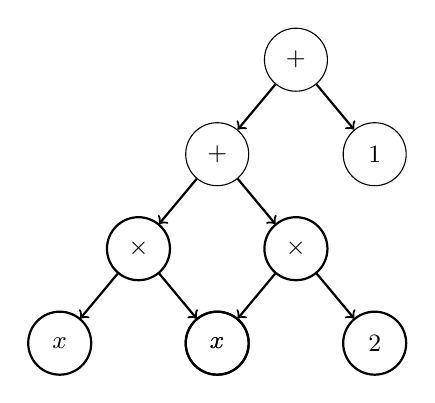
\begin{tikzpicture}[
    level distance=1.2cm,
    sibling distance=2cm,
    every node/.style={draw, circle, minimum size=0.8cm, font=\small},
    edge from parent/.style={draw, ->, thick}
]
    \node {$+$}
        child { node {$+$}
            child { node {$\times$}
                child { node {$x$} }
                child { node {$x$} }
            }
            child { node {$\times$}
                child { node {$x$} }
                child { node {$2$} }
            }
        }
        child { node {$1$} };
\end{tikzpicture}
\end{center}

这棵树的结构就是 $(((x \times x) + (x \times 2)) + 1)$。\textbf{``先乘后加''是在这一步决定的}。

\paragraph{第二步：编译（Compilation）—— 把树变成指令序列}

Python 编译器把 AST 翻译成一串\textbf{字节码指令}（bytecode）。每条指令只做一件很小的事：

\begin{center}
\renewcommand{\arraystretch}{1.3}
\begin{tabular}{cl}
\toprule
\textbf{指令} & \textbf{含义} \\
\midrule
\texttt{LOAD\_FAST x} & 把变量 $x$ 压入栈顶 \\
\texttt{BINARY\_MULTIPLY} & 弹出栈顶两个数，相乘，结果压回栈顶 \\
\texttt{BINARY\_ADD} & 弹出栈顶两个数，相加，结果压回栈顶 \\
\texttt{LOAD\_CONST 2} & 把常数 2 压入栈顶 \\
\bottomrule
\end{tabular}
\end{center}

\paragraph{第三步：执行（Execution）—— 用栈依次运行指令}

解释器维护一个\textbf{栈}（像一摞盘子），严格按字节码顺序执行：

\begin{center}
\renewcommand{\arraystretch}{1.4}
\begin{tabular}{c|l|l}
\toprule
\textbf{步骤} & \textbf{执行的指令} & \textbf{栈的状态}（右边是栈顶） \\
\midrule
1 & \texttt{LOAD\_FAST x} & $[3.0]$ \\
2 & \texttt{LOAD\_FAST x} & $[3.0, 3.0]$ \\
3 & \texttt{BINARY\_MULTIPLY} $\to$ 调用 \texttt{x.\_\_mul\_\_(x)} & $[m_1]$ \quad ($m_1$.data=9.0) \\
\midrule
4 & \texttt{LOAD\_FAST x} & $[m_1, 3.0]$ \\
5 & \texttt{LOAD\_CONST 2} & $[m_1, 3.0, 2]$ \\
6 & \texttt{BINARY\_MULTIPLY} $\to$ 调用 \texttt{x.\_\_mul\_\_(2)} & $[m_1, m_2]$ \quad ($m_2$.data=6.0) \\
\midrule
7 & \texttt{BINARY\_ADD} $\to$ 调用 \texttt{m1.\_\_add\_\_(m2)} & $[s_1]$ \quad ($s_1$.data=15.0) \\
\midrule
8 & \texttt{LOAD\_CONST 1} & $[s_1, 1]$ \\
9 & \texttt{BINARY\_ADD} $\to$ 调用 \texttt{s1.\_\_add\_\_(1)} & $[y]$ \quad ($y$.data=16.0) \\
\bottomrule
\end{tabular}
\end{center}

\textbf{关键洞察}：每次执行 \texttt{BINARY\_MULTIPLY} 或 \texttt{BINARY\_ADD} 时，Python 会调用我们重载的 \texttt{\_\_mul\_\_} 或 \texttt{\_\_add\_\_} 方法。在这些方法里，我们不仅计算了数值，还\textbf{顺便}创建了计算图节点！

\subsection*{真的可以看到字节码吗？}

可以！Python 提供了 \texttt{dis} 模块来查看字节码：

\begin{lstlisting}[style=teaching, language=Python]
import dis

def f(x):
    return x * x + x * 2 + 1

dis.dis(f)
\end{lstlisting}

输出（简化后）：

\begin{lstlisting}[style=teaching, language=Python, numbers=none]
  3           0 LOAD_FAST                0 (x)
              2 LOAD_FAST                0 (x)
              4 BINARY_MULTIPLY              # x * x -> m1

              6 LOAD_FAST                0 (x)
              8 LOAD_CONST               1 (2)
             10 BINARY_MULTIPLY              # x * 2 -> m2

             12 BINARY_ADD                   # m1 + m2 -> s1

             14 LOAD_CONST               2 (1)
             16 BINARY_ADD                   # s1 + 1 -> y

             18 RETURN_VALUE
\end{lstlisting}

这正是我们前面 Step 1--4 图的``官方版本''！

\subsection*{小结}

\begin{center}
\begin{tikzpicture}[
    box/.style={draw, rounded corners, minimum width=3cm, minimum height=1cm, font=\small, align=center},
    arrow/.style={->, thick, >=stealth}
]
    \node[box, fill=blue!10] (src) at (0, 0) {源代码\\{\ttfamily x*x + x*2 + 1}};
    \node[box, fill=green!10] (ast) at (4.5, 0) {抽象语法树\\（确定优先级）};
    \node[box, fill=yellow!10] (bc) at (9, 0) {字节码序列\\（线性指令）};
    \node[box, fill=red!10] (exec) at (13.5, 0) {栈式执行\\（调用重载方法）};
    
    \draw[arrow] (src) -- node[above, font=\scriptsize] {解析} (ast);
    \draw[arrow] (ast) -- node[above, font=\scriptsize] {编译} (bc);
    \draw[arrow] (bc) -- node[above, font=\scriptsize] {执行} (exec);
\end{tikzpicture}
\end{center}

\begin{itemize}
    \item \textbf{``先乘后加''}是在\textbf{解析阶段}决定的（构建 AST）
    \item \textbf{``从左到右''}是在\textbf{执行阶段}实现的（按字节码顺序）
    \item \textbf{我们没有写任何解析器}，Python 帮我们做完了所有这些工作
    \item 我们只需要\textbf{重载运算符}，就能在执行阶段``搭便车''构建计算图
\end{itemize}

这就是自动微分框架的设计哲学：\textbf{利用宿主语言的表达式求值机制，免费获得计算图构建能力}。PyTorch、JAX、TensorFlow Eager 都是这个思路。

\section*{扩展阅读：深度学习与数值方法的深刻联系——第5章的后续}
\addcontentsline{toc}{section}{扩展阅读：与数值方法的联系}

\marginnote{这一节揭示深度学习与经典数值方法的内在联系。你会发现，很多``新''的深度学习技术，其实是老方法的新面孔。}

深度学习中的许多核心概念，与数值线性代数、有限元方法有着惊人的相似性。理解这些联系，能帮助你更深刻地理解两个领域。

\subsection*{条件数与训练困难}

梯度下降的收敛速度取决于损失函数的\textbf{Hessian矩阵}（二阶导数矩阵）的\textbf{条件数}。

\begin{definition}[Hessian 矩阵]
Hessian 矩阵 $H$ 是损失函数的二阶偏导数组成的矩阵：
\begin{equation}
H_{ij} = \frac{\partial^2 L}{\partial \theta_i \partial \theta_j}
\end{equation}
它描述了损失曲面的``曲率''——在不同方向上曲面弯曲的程度。
\end{definition}

\begin{figure}[h]
\centering
\begin{tikzpicture}[scale=0.75]
    % 良态：接近圆形
    \begin{scope}
        \node[font=\bfseries] at (2, 3.8) {良态（$\kappa \approx 1$）};
        \draw[->] (0, 0) -- (4, 0) node[right] {$\theta_1$};
        \draw[->] (0, 0) -- (0, 3.2) node[above] {$\theta_2$};
        
        % 等高线（接近圆形）
        \draw[blue!40] (2, 1.5) ellipse (1.4 and 1.2);
        \draw[blue!60] (2, 1.5) ellipse (0.9 and 0.75);
        \draw[blue!80] (2, 1.5) ellipse (0.4 and 0.33);
        \fill[red] (2, 1.5) circle (2pt);
        
        % 梯度下降路径
        \draw[->, thick, red] (0.8, 2.5) -- (1.5, 1.8) -- (1.9, 1.55) -- (2, 1.5);
        
        \node[font=\small] at (2, -0.5) {各方向曲率相近 $\to$ 快速收敛};
    \end{scope}
    
    % 病态：扁椭圆
    \begin{scope}[xshift=6.5cm]
        \node[font=\bfseries] at (2, 3.8) {病态（$\kappa \gg 1$）};
        \draw[->] (0, 0) -- (4, 0) node[right] {$\theta_1$};
        \draw[->] (0, 0) -- (0, 3.2) node[above] {$\theta_2$};
        
        % 等高线（扁椭圆）
        \draw[blue!40, rotate around={20:(2,1.5)}] (2, 1.5) ellipse (1.6 and 0.35);
        \draw[blue!60, rotate around={20:(2,1.5)}] (2, 1.5) ellipse (1.0 and 0.22);
        \draw[blue!80, rotate around={20:(2,1.5)}] (2, 1.5) ellipse (0.4 and 0.09);
        \fill[red] (2, 1.5) circle (2pt);
        
        % 梯度下降路径（锯齿）
        \draw[->, thick, red] (3.5, 2.3) -- (2.5, 1.2) -- (3.0, 1.7) -- (2.3, 1.3) -- (2.6, 1.55) -- (2.2, 1.4);
        
        \node[font=\small] at (2, -0.5) {曲率差异大 $\to$ 锯齿震荡};
    \end{scope}
\end{tikzpicture}
\caption{条件数决定损失曲面的``形状''：圆形容易优化，扁椭圆困难}
\end{figure}

\begin{itemize}
    \item \textbf{$\kappa$ 小}：各方向曲率相近，等高线接近圆形，梯度直指最低点
    \item \textbf{$\kappa$ 大}：有的方向很陡，有的方向很平，梯度下降会在陡峭方向来回震荡
\end{itemize}

这与求解线性方程组 $Ax = b$ 时的情况完全一致！

\subsection*{优化器 = 预条件子}

几乎所有现代优化器都可以理解为某种\textbf{预条件}（preconditioning）！

\begin{center}
\renewcommand{\arraystretch}{1.4}
\begin{tabular}{l|l|l}
\toprule
\textbf{数值线性代数} & \textbf{深度学习优化器} & \textbf{预条件矩阵 $M$} \\
\midrule
无预条件 & SGD & $M = I$ \\
Jacobi 预条件 & Adagrad / RMSprop & $M = \text{diag}(\sqrt{v})$ \\
近似 Newton 法 & Adam & $M = \text{diag}(\sqrt{\hat{v}})$ \\
完整 Newton 法 & K-FAC, Shampoo & $M \approx H$ \\
\bottomrule
\end{tabular}
\end{center}

\textbf{Adam 的本质}：用对角预条件子对梯度进行缩放：
\begin{equation}
\theta^{(t+1)} = \theta^{(t)} - \eta \cdot \frac{\hat{m}}{\sqrt{\hat{v}} + \epsilon} = \theta^{(t)} - \eta \cdot M^{-1} \hat{m}
\end{equation}

\begin{itemize}
    \item 梯度大的方向（$\hat{v}$ 大）：步长缩小，防止震荡
    \item 梯度小的方向（$\hat{v}$ 小）：步长放大，加速收敛
\end{itemize}

这与数值线性代数中的 Jacobi 预条件思想完全一致！

\subsection*{稀疏性：从有限元到卷积网络}

有限元刚度矩阵是\textbf{稀疏}的（每个节点只与邻居耦合），现代神经网络也追求稀疏性。

\begin{figure}[h]
\centering
\begin{tikzpicture}[scale=0.8]
    % 左边：全连接
    \begin{scope}
        \node[font=\bfseries] at (1.5, 4) {全连接层};
        % 输入节点
        \foreach \i in {1,...,4} {
            \fill[blue] (0, \i) circle (4pt);
        }
        % 输出节点
        \foreach \i in {1,...,3} {
            \fill[red] (3, \i+0.5) circle (4pt);
        }
        % 连接
        \foreach \i in {1,...,4} {
            \foreach \j in {1,...,3} {
                \draw[gray, thin] (0, \i) -- (3, \j+0.5);
            }
        }
        \node[font=\small] at (1.5, 0.3) {$O(n \times m)$ 参数};
    \end{scope}
    
    % 右边：稀疏连接（卷积）
    \begin{scope}[xshift=6cm]
        \node[font=\bfseries] at (1.5, 4) {卷积层};
        % 输入节点
        \foreach \i in {1,...,4} {
            \fill[blue] (0, \i) circle (4pt);
        }
        % 输出节点
        \foreach \i in {1,...,3} {
            \fill[red] (3, \i+0.5) circle (4pt);
        }
        % 局部连接
        \draw[thick] (0, 1) -- (3, 1.5);
        \draw[thick] (0, 2) -- (3, 1.5);
        \draw[thick] (0, 2) -- (3, 2.5);
        \draw[thick] (0, 3) -- (3, 2.5);
        \draw[thick] (0, 3) -- (3, 3.5);
        \draw[thick] (0, 4) -- (3, 3.5);
        \node[font=\small] at (1.5, 0.3) {$O(k)$ 参数};
    \end{scope}
\end{tikzpicture}
\caption{全连接层 vs 卷积层：稀疏连接大幅减少参数}
\end{figure}

\textbf{卷积神经网络（CNN）}利用了与有限元相同的原理：

\begin{itemize}
    \item \textbf{局部连接}：每个输出只依赖局部输入（类比：每个节点只与邻居耦合）
    \item \textbf{权值共享}：不同位置用相同的卷积核（类比：均匀网格上的单元刚度矩阵相同）
    \item \textbf{稀疏性}：参数量从 $O(n^2)$ 降到 $O(n)$
\end{itemize}

\begin{insightbox}[title=局部性的力量]
有限元方法和卷积神经网络都在利用\textbf{局部性}——物理世界的大多数相互作用是局部的：
\begin{itemize}
    \item 热量从高温流向低温（局部传导）
    \item 力通过接触传递（局部作用）
    \item 图像特征是局部的（边缘、纹理）
\end{itemize}
局部性导致稀疏结构，稀疏结构带来计算上的巨大节省！
\end{insightbox}

\subsection*{多重网格与 U-Net}

数值方法中的\textbf{多重网格}（multigrid）技术在深度学习中有惊人的对应物：\textbf{U-Net}！

\begin{figure}[h]
\centering
\begin{tikzpicture}[scale=0.65]
    % U-Net 结构
    % 左边：编码器（下采样）
    \draw[fill=blue!30] (0, 0) rectangle (1.5, 4);
    \node[font=\scriptsize] at (0.75, 2) {细};
    \draw[fill=blue!40] (2, 0.5) rectangle (3, 3.5);
    \draw[fill=blue!50] (3.5, 1) rectangle (4.5, 3);
    \draw[fill=blue!60] (5, 1.5) rectangle (5.5, 2.5);
    \node[font=\scriptsize] at (5.25, 2) {粗};
    
    % 右边：解码器（上采样）
    \draw[fill=red!30] (9, 0) rectangle (10.5, 4);
    \node[font=\scriptsize] at (9.75, 2) {细};
    \draw[fill=red!40] (7.5, 0.5) rectangle (8.5, 3.5);
    \draw[fill=red!50] (6, 1) rectangle (7, 3);
    
    % 跳跃连接
    \draw[->, thick, green!60!black] (1.5, 3.5) to[bend left=20] (9, 3.5);
    \draw[->, thick, green!60!black] (3, 3) to[bend left=15] (7.5, 3);
    \draw[->, thick, green!60!black] (4.5, 2.5) to[bend left=10] (6, 2.5);
    
    % 箭头
    \draw[->, thick] (1.6, 2) -- (1.9, 2);
    \draw[->, thick] (3.1, 2) -- (3.4, 2);
    \draw[->, thick] (4.6, 2) -- (4.9, 2);
    \draw[->, thick] (5.6, 2) -- (5.9, 2);
    \draw[->, thick] (7.1, 2) -- (7.4, 2);
    \draw[->, thick] (8.6, 2) -- (8.9, 2);
    
    % 标签
    \node at (2.5, 4.8) {下采样（限制）};
    \node at (7.5, 4.8) {上采样（插值）};
    \node[green!60!black, font=\small] at (5.25, 4.3) {跳跃连接};
\end{tikzpicture}
\caption{U-Net 结构与多重网格的惊人相似}
\end{figure}

\begin{center}
\renewcommand{\arraystretch}{1.4}
\begin{tabular}{l|l}
\toprule
\textbf{多重网格} & \textbf{U-Net} \\
\midrule
限制（Restriction） & 池化 / 下采样 \\
粗网格求解 & 瓶颈层处理 \\
插值（Prolongation） & 转置卷积 / 上采样 \\
粗细网格信息传递 & 跳跃连接（Skip Connection） \\
\bottomrule
\end{tabular}
\end{center}

U-Net 在医学图像分割等任务中非常成功——它继承了多重网格``多尺度处理''的智慧！

\subsection*{GPU 并行：为什么深度学习需要 GPU}

深度学习的爆发离不开 \textbf{GPU}，而 GPU 擅长的恰恰是\textbf{大规模并行计算}。

\begin{figure}[h]
\centering
\begin{tikzpicture}[scale=0.8]
    % CPU
    \begin{scope}
        \node[font=\bfseries] at (1.6, 2.8) {CPU};
        \foreach \i in {0,...,3} {
            \draw[fill=blue!50] (\i*0.8, 0) rectangle ++(0.7, 0.7);
        }
        \node[font=\small] at (1.6, -0.5) {4--16 个强核心};
        \node[font=\small] at (1.6, -1) {擅长复杂逻辑};
    \end{scope}
    
    % GPU
    \begin{scope}[xshift=6cm]
        \node[font=\bfseries] at (2.4, 2.8) {GPU};
        \foreach \i in {0,...,9} {
            \foreach \j in {0,...,3} {
                \draw[fill=green!50] (\i*0.5, \j*0.5) rectangle ++(0.4, 0.4);
            }
        }
        \node[font=\small] at (2.4, -0.5) {数千个小核心};
        \node[font=\small] at (2.4, -1) {擅长简单并行};
    \end{scope}
\end{tikzpicture}
\caption{CPU vs GPU：不同的设计哲学}
\end{figure}

\textbf{为什么神经网络适合 GPU？}

神经网络的核心运算是\textbf{矩阵乘法}：$Y = XW + b$。

矩阵乘法中，每个输出元素 $Y_{ij} = \sum_k X_{ik} W_{kj}$ 可以\textbf{独立计算}——这是天然的并行结构！

\begin{insightbox}[title=GPU 友好的计算模式]
\begin{enumerate}
    \item \textbf{大量独立的相同操作}（如 batch 中每个样本的前向传播）
    \item \textbf{规则的内存访问}（如矩阵乘法的连续读写）
    \item \textbf{少量分支逻辑}（避免 if-else 导致的线程分化）
\end{enumerate}

这解释了为什么：
\begin{itemize}
    \item Transformer 比 RNN 更容易并行（无时序依赖）
    \item 卷积比全连接更高效（局部性好，缓存友好）
    \item Batch Normalization 比 Layer Normalization 更 GPU 友好
\end{itemize}
\end{insightbox}

\subsection*{统一的视角}

回顾本章和这些扩展阅读，我们看到一个统一的图景：

\begin{center}
\renewcommand{\arraystretch}{1.5}
\begin{tabular}{l|l|l}
\toprule
\textbf{概念} & \textbf{数值方法} & \textbf{深度学习} \\
\midrule
核心问题 & 求解 $Ax = b$ 或 $\min_x f(x)$ & 求解 $\min_\theta L(\theta)$ \\
迭代方法 & Jacobi, Gauss-Seidel, CG & SGD, Momentum, Adam \\
加速技术 & 预条件子 & 自适应学习率 \\
利用结构 & 稀疏矩阵 & 卷积、注意力 \\
多尺度 & 多重网格 & U-Net, Feature Pyramid \\
并行化 & 区域分解 & 数据并行、模型并行 \\
\bottomrule
\end{tabular}
\end{center}

\textbf{核心信息}：深度学习不是凭空出现的``黑魔法''，而是建立在几十年数值计算研究基础上的自然延伸。理解经典方法，能帮助你更好地理解和改进现代深度学习技术。

\section*{扩展阅读：深度学习的计算基础设施}
\addcontentsline{toc}{section}{扩展阅读：计算基础设施}

当你写下 \texttt{y = torch.matmul(A, B)} 时，背后发生了什么？为什么 GPU 
比 CPU 快 100 倍？为了理解这一点，我们先从一个经典的小故事开始。

\subsection*{一个被认为“毫无意义”的实验}

\marginnote{\textbf{Geoffrey Hinton}(1947--)：``深度学习教父''，2018年图灵奖得主。他在多伦多大学坚持神经网络研究三十年，在AI冬天时几乎是孤军奋战。2012年AlexNet的成功证明了他的坚持。2023年他辞去Google职位，公开警告AI的潜在危险。}

2009 年，Montreal 的一间小实验室里，博士生 Ranzato、
助手 Alex Krizhevsky，以及他们的导师 Hinton 正在做一个
很多人看来``一点用都没有''的实验——

\begin{quote}
用当时游戏玩家的显卡（NVIDIA GTX 280）来训练一个
卷积神经网络。
\end{quote}

在那个年代，深度学习还远没有今天的气势。主流观点认为：

\begin{itemize}
    \item 深度网络太大，训练太慢；
    \item GPU 只是玩游戏的，没有科研价值；
    \item 机器学习的未来应该是从数学上给模型加约束，而不是暴力堆算力。
\end{itemize}

但 Krizhevsky 注意到了一件别人忽略的事：  
游戏显卡的核心结构（SIMD + 大量并行浮点单元）和卷积操作的数学结构是完美匹配的。

于是他们写下了第一版用 CUDA 加速卷积的代码，
发现速度比 CPU \textbf{快了几十倍}。Hinton 后来回忆说：

\begin{quote}
``第一次看到 GPU 把卷积层跑得这么快时，我们觉得好像未来突然被打开了。''
\end{quote}

三年后，也就是 2012 年，Krizhevsky 基于这些经验写出了 \texttt{cuda-convnet}，并用一台双 GTX 580 显卡训练出了历史性的模型——

\begin{center}
\textbf{AlexNet}
\end{center}

它把 ImageNet 错误率降低了 10 个百分点，直接点燃了整个深度学习时代。

从此之后，一个事实被彻底确认：

\begin{quote}
\textbf{深度学习的突破，离不开硬件架构与数学结构的完美匹配。}
\end{quote}

而你今天执行的 \texttt{torch.matmul}、\texttt{conv2d} 等操作，
本质上都是在 GPU 上调用几十年积累下来的线性代数内核（cuBLAS、cuDNN），
这些内核又精确地利用了 GPU 的大规模并行结构。

因此，表面上一行 Python：

\begin{equation}
y = \text{torch.matmul}(A, B)
\end{equation}

背后是一整套工业级的软硬件生态：计算图编译器、Tensor Core、
warp 调度、内存对齐、缓存优化、并行线程块调度……

理解这一点后，PyTorch 为什么快，就不再是魔法，而是工程与数学共同的必然结果(这一节以英伟达NVIDIA相关生态举例，华为等硬件厂商也有类似的底层架构逻辑，机器码和线程管理模式不尽相同)。

\subsection*{GPU 编程的层次结构}

深度学习的计算栈是这样的：

\begin{figure}[h]
\centering
\begin{tikzpicture}[
    box/.style={draw, rounded corners, minimum width=4cm, minimum height=0.9cm, font=\small, align=center},
    arrow/.style={->, thick, >=stealth}
]
    \node[box, fill=blue!20] (python) at (0, 5) {Python 代码\\{\ttfamily y = model(x)}};
    \node[box, fill=blue!30] (pytorch) at (0, 3.8) {PyTorch / JAX / TensorFlow\\自动微分、张量操作};
    \node[box, fill=green!20] (cuda) at (0, 2.6) {CUDA / cuDNN / cuBLAS\\GPU 算子库};
    \node[box, fill=yellow!20] (driver) at (0, 1.4) {GPU 驱动\\内存管理、任务调度};
    \node[box, fill=red!20] (hw) at (0, 0.2) {GPU 硬件\\CUDA Core / Tensor Core};
    
    \draw[arrow] (python) -- (pytorch);
    \draw[arrow] (pytorch) -- (cuda);
    \draw[arrow] (cuda) -- (driver);
    \draw[arrow] (driver) -- (hw);
    
    % 右侧标注
    \node[right, font=\small, text=gray] at (2.3, 5) {你写的};
    \node[right, font=\small, text=gray] at (2.3, 3.8) {框架提供};
    \node[right, font=\small, text=gray] at (2.3, 2.6) {NVIDIA 提供};
    \node[right, font=\small, text=gray] at (2.3, 1.4) {系统层};
    \node[right, font=\small, text=gray] at (2.3, 0.2) {硬件层};
\end{tikzpicture}
\caption{深度学习计算栈：从 Python 到硬件}
\end{figure}

\subsection*{CUDA：GPU 编程的基础}

\textbf{CUDA}（Compute Unified Device Architecture）是 NVIDIA 的 GPU 编程平台。

\paragraph{核心概念}

\begin{itemize}
    \item \textbf{Thread}：最小执行单元，执行相同的代码（SIMT: Single Instruction Multiple Threads）
    \item \textbf{Block}：一组线程，共享高速的 Shared Memory
    \item \textbf{Grid}：所有 Block 的集合，完成一个计算任务
\end{itemize}

\begin{figure}[h]
\centering
\begin{tikzpicture}[scale=0.8]
    % Grid
    \draw[thick, blue] (0, 0) rectangle (8, 4);
    \node[blue, font=\bfseries] at (4, 4.4) {Grid（整个任务）};
    
    % Blocks
    \foreach \i in {0, 2.7, 5.4} {
        \draw[thick, green!60!black, fill=green!10] (\i+0.2, 0.2) rectangle (\i+2.5, 3.8);
    }
    \node[green!60!black, font=\small] at (1.35, 3.5) {Block 0};
    \node[green!60!black, font=\small] at (4.05, 3.5) {Block 1};
    \node[green!60!black, font=\small] at (6.75, 3.5) {Block 2};
    
    % Threads in first block
    \foreach \i in {0,...,3} {
        \foreach \j in {0,...,2} {
            \draw[fill=red!30] (0.4+\i*0.5, 0.5+\j*0.9) rectangle ++(0.4, 0.7);
        }
    }
    \node[font=\scriptsize] at (1.35, 0.3) {Threads};
    
    % 标注
    \node[right, font=\small, align=left] at (8.5, 3) {每个 Block：\\共享 Shared Memory\\同步执行};
    \node[right, font=\small, align=left] at (8.5, 1) {每个 Thread：\\独立寄存器\\执行相同代码};
\end{tikzpicture}
\caption{CUDA 的线程层次：Grid → Block → Thread}
\end{figure}

\paragraph{一个简单的 CUDA 核函数}

\begin{lstlisting}[style=teaching, language=C]
// 向量加法的 CUDA 实现
__global__ void vector_add(float *a, float *b, float *c, int n) {
    // 计算当前线程负责的元素索引
    int idx = blockIdx.x * blockDim.x + threadIdx.x;
    
    if (idx < n) {
        c[idx] = a[idx] + b[idx];  // 每个线程只算一个元素！
    }
}

// 调用：启动 N 个线程并行计算
vector_add<<<num_blocks, threads_per_block>>>(a, b, c, N);
\end{lstlisting}

\textbf{关键洞察}：传统 CPU 代码用 \texttt{for} 循环遍历数组，CUDA 代码让每个线程只处理一个元素，成千上万个线程\textbf{同时}执行！

\subsection*{内存层次与性能优化}

GPU 有多级内存，访问速度差异巨大：

\begin{center}
\renewcommand{\arraystretch}{1.4}
\begin{tabular}{l|r|r|l}
\toprule
\textbf{内存类型} & \textbf{大小} & \textbf{带宽} & \textbf{延迟} \\
\midrule
寄存器（Register） & $\sim$256 KB/SM & -- & 1 cycle \\
共享内存（Shared Memory） & $\sim$100 KB/SM & $\sim$19 TB/s & $\sim$20 cycles \\
L2 缓存 & $\sim$40 MB & $\sim$6 TB/s & $\sim$200 cycles \\
全局内存（Global/HBM） & 24--80 GB & $\sim$2 TB/s & $\sim$400 cycles \\
\bottomrule
\end{tabular}
\end{center}

\marginnote{SM = Streaming Multiprocessor，GPU 的计算单元。一个 GPU 有几十到上百个 SM。}

\textbf{性能优化的核心}：尽量让数据停留在快速的内存层次中！

\begin{itemize}
    \item \textbf{访存合并}（Memory Coalescing）：相邻线程访问相邻内存，一次传输搞定
    \item \textbf{Shared Memory}：Block 内的线程共享数据，避免重复读取全局内存
    \item \textbf{寄存器复用}：计算密集型操作尽量用寄存器存中间结果
\end{itemize}

\subsection*{张量的内存布局：Stride 的秘密}

当你创建一个 PyTorch 张量时，它在内存中是怎么存储的？

\begin{lstlisting}[style=teaching, language=Python]
import torch

A = torch.tensor([[1, 2, 3],
                  [4, 5, 6]])  # shape: (2, 3)

print(A.storage())  # 底层存储：[1, 2, 3, 4, 5, 6]（一维数组！）
print(A.stride())   # 步长：(3, 1)
\end{lstlisting}

\textbf{Stride}（步长）告诉我们：沿每个维度移动一步，需要在底层数组中跳过多少元素。

\begin{figure}[h]
\centering
\begin{tikzpicture}[scale=0.9]
    % 底层一维数组
    \foreach \i/\v in {0/1, 1/2, 2/3, 3/4, 4/5, 5/6} {
        \draw[fill=blue!20] (\i*1.2, 0) rectangle ++(1, 0.8);
        \node at (\i*1.2+0.5, 0.4) {\v};
        \node[font=\scriptsize, gray] at (\i*1.2+0.5, -0.3) {\i};
    }
    \node[font=\small] at (3.5, -0.8) {底层存储（连续内存）};
    
    % 逻辑视图
    \node at (-1.5, 2.5) {逻辑视图：};
    \draw[fill=green!20] (0, 2) rectangle ++(1, 0.8); \node at (0.5, 2.4) {1};
    \draw[fill=green!20] (1.2, 2) rectangle ++(1, 0.8); \node at (1.7, 2.4) {2};
    \draw[fill=green!20] (2.4, 2) rectangle ++(1, 0.8); \node at (2.9, 2.4) {3};
    \draw[fill=green!20] (0, 3) rectangle ++(1, 0.8); \node at (0.5, 3.4) {4};
    \draw[fill=green!20] (1.2, 3) rectangle ++(1, 0.8); \node at (1.7, 3.4) {5};
    \draw[fill=green!20] (2.4, 3) rectangle ++(1, 0.8); \node at (2.9, 3.4) {6};
    
    % stride 标注
    \draw[<->, thick, red] (0.5, 1.8) -- (0.5, 1.2) -- (3.5, 1.2) -- (3.5, 0.9);
    \node[red, font=\small] at (2, 1.5) {stride[0]=3};
    
    \draw[<->, thick, orange] (4.5, 2.4) -- (5.5, 2.4);
    \node[orange, font=\small] at (5, 2.8) {stride[1]=1};
\end{tikzpicture}
\caption{张量的 Stride：逻辑多维数组如何映射到一维内存}
\end{figure}

\paragraph{为什么 Stride 重要？}

\textbf{转置}不需要复制数据，只需要交换 stride！

\begin{lstlisting}[style=teaching, language=Python]
A = torch.tensor([[1, 2, 3],
                  [4, 5, 6]])
print(A.stride())       # (3, 1) - 行优先

B = A.T                 # 转置
print(B.stride())       # (1, 3) - 列优先
print(B.storage())      # 还是 [1, 2, 3, 4, 5, 6]，没有复制！

# 但是 B 不是"连续"的
print(B.is_contiguous())  # False
\end{lstlisting}

\begin{insightbox}[title=Contiguous 的含义]
一个张量是 \textbf{contiguous} 的，当且仅当它的内存布局与从头创建时一致（行优先，stride 递减）。

很多 CUDA 算子要求输入是 contiguous 的，否则需要先调用 \texttt{.contiguous()} 复制一份数据。这是常见的性能陷阱！
\end{insightbox}

\subsection*{cuBLAS 和 cuDNN：优化到极致的算子库}

自己写 CUDA 核函数很难达到最优性能。NVIDIA 提供了高度优化的库：

\begin{itemize}
    \item \textbf{cuBLAS}：基础线性代数（矩阵乘法、向量运算）
    \item \textbf{cuDNN}：深度学习原语（卷积、BatchNorm、RNN）
    \item \textbf{cuFFT}：快速傅里叶变换
    \item \textbf{cuSPARSE}：稀疏矩阵运算
\end{itemize}

\textbf{矩阵乘法有多复杂？}
\marginnote{一个优化良好的矩阵乘法实现可能有上万行代码，针对不同尺寸有几十个特化版本。}

看似简单的 $C = AB$，cuBLAS 的实现考虑了：
\begin{itemize}
    \item 矩阵分块（Tiling）：适配 Shared Memory 大小
    \item 数据预取（Prefetching）：隐藏内存延迟
    \item 向量化访存：一次读取 128 位
    \item Tensor Core 加速：专用硬件做 $4 \times 4$ 矩阵乘
    \item 不同矩阵尺寸的特化实现
\end{itemize}



\subsection*{Triton：让 GPU 编程更简单}

\textbf{Triton} 是由 OpenAI 推出的新一代 GPU 编程语言，旨在让研究者能够\textbf{以接近 Python 的方式编写高性能的自定义算子}，而无需深度掌握 CUDA 的底层细节。它在矩阵乘法、注意力等核心算子上曾展现出与手写 CUDA 相当甚至更优的性能。由于长期维护成本高、生态兼容性复杂，Triton 已于 2025 年 11 月正式停止维护，但其思想（如自动优化、块级并行抽象）仍然对后续深度学习编译器的设计产生了重要影响。

\begin{lstlisting}[style=teaching, language=Python]
import triton
import triton.language as tl

@triton.jit
def vector_add_kernel(x_ptr, y_ptr, out_ptr, n, BLOCK_SIZE: tl.constexpr):
    # 每个程序实例处理 BLOCK_SIZE 个元素
    pid = tl.program_id(0)
    offsets = pid * BLOCK_SIZE + tl.arange(0, BLOCK_SIZE)
    mask = offsets < n
    
    # 向量化加载、计算、存储
    x = tl.load(x_ptr + offsets, mask=mask)
    y = tl.load(y_ptr + offsets, mask=mask)
    tl.store(out_ptr + offsets, x + y, mask=mask)
\end{lstlisting}

\textbf{Triton vs CUDA}：

\begin{center}
\renewcommand{\arraystretch}{1.4}
\begin{tabular}{l|l|l}
\toprule
\textbf{方面} & \textbf{CUDA} & \textbf{Triton} \\
\midrule
语言 & C++ 扩展 & Python 风格 \\
抽象层次 & 线程级 & Block 级 \\
内存管理 & 手动 & 自动 Tiling \\
性能调优 & 繁琐 & 编译器自动优化 \\
学习曲线 & 陡峭 & 相对平缓 \\
\bottomrule
\end{tabular}
\end{center}

PyTorch 2.0 的 \texttt{torch.compile} 就使用 Triton 生成高效的融合算子。

\subsection*{算子融合：减少内存访问}

深度学习中一个关键优化是\textbf{算子融合}（Kernel Fusion）。

考虑 $y = \text{ReLU}(Wx + b)$，朴素实现：

\begin{lstlisting}[style=teaching, language=Python]
# 朴素实现：3 次 kernel launch，3 次读写全局内存
z1 = torch.matmul(W, x)   # 写 z1 到 HBM
z2 = z1 + b               # 读 z1，写 z2 到 HBM  
y = torch.relu(z2)        # 读 z2，写 y 到 HBM
\end{lstlisting}

\textbf{问题}：每个操作都要把中间结果写回慢速的全局内存（HBM），再读出来。

\textbf{融合后}：一个 kernel 完成所有操作，中间结果只在寄存器/Shared Memory 中：

\begin{lstlisting}[style=teaching, language=Python]
# 融合实现：1 次 kernel launch，中间结果不写回 HBM
@triton.jit
def fused_linear_relu(x, W, b, y, ...):
    z1 = dot(W, x)        # 结果在寄存器
    z2 = z1 + b           # 结果在寄存器
    y = max(z2, 0)        # 直接写最终结果
\end{lstlisting}

\begin{figure}[h]
\centering
\begin{tikzpicture}[scale=0.8]
    % 朴素版本
    \begin{scope}
        \node[font=\bfseries] at (2, 4) {朴素实现};
        \draw[fill=green!20] (0, 3) rectangle (1.5, 3.5); \node[font=\small] at (0.75, 3.25) {matmul};
        \draw[fill=green!20] (2, 3) rectangle (3.5, 3.5); \node[font=\small] at (2.75, 3.25) {add};
        \draw[fill=green!20] (4, 3) rectangle (5.5, 3.5); \node[font=\small] at (4.75, 3.25) {relu};
        
        \draw[fill=red!20] (0, 1.5) rectangle (5.5, 2.2);
        \node[font=\small] at (2.75, 1.85) {HBM（全局内存）};
        
        \draw[->, thick] (0.75, 3) -- (0.75, 2.2);
        \draw[->, thick] (0.75, 2.2) -- (2.75, 2.2) -- (2.75, 3);
        \draw[->, thick] (2.75, 3) -- (2.75, 2.2);
        \draw[->, thick] (2.75, 2.2) -- (4.75, 2.2) -- (4.75, 3);
        
        \node[font=\small, red] at (2.75, 0.8) {6 次 HBM 访问};
    \end{scope}
    
    % 融合版本
    \begin{scope}[xshift=8cm]
        \node[font=\bfseries] at (2, 4) {融合实现};
        \draw[fill=blue!30] (0.5, 2.8) rectangle (4, 3.7);
        \node[font=\small] at (2.25, 3.25) {fused\_linear\_relu};
        
        \draw[fill=yellow!30] (1, 2) rectangle (3.5, 2.5);
        \node[font=\small] at (2.25, 2.25) {寄存器};
        
        \draw[fill=red!20] (0, 0.8) rectangle (4.5, 1.3);
        \node[font=\small] at (2.25, 1.05) {HBM};
        
        \draw[->, thick, dashed] (2.25, 2.8) -- (2.25, 2.5);
        \draw[->, thick] (2.25, 2) -- (2.25, 1.3);
        
        \node[font=\small, blue] at (2.25, 0.3) {1 次 HBM 写入};
    \end{scope}
\end{tikzpicture}
\caption{算子融合减少内存访问：6 次 $\to$ 1 次}
\end{figure}

FlashAttention 就是通过融合 QKV 计算、Softmax、输出投影，避免了存储巨大的注意力矩阵。

\subsection*{深度学习软件生态}

\begin{figure}[h]
\centering
\begin{tikzpicture}[
    box/.style={draw, rounded corners, minimum height=0.8cm, font=\small, align=center},
    scale=0.85, transform shape
]
    % 应用层
    \node[box, fill=purple!20, minimum width=8cm] at (4, 5) {应用：ChatGPT, Stable Diffusion, AlphaFold};
    
    % 框架层
    \node[box, fill=blue!20, minimum width=2.4cm] at (1.2, 4) {PyTorch};
    \node[box, fill=blue!20, minimum width=2.4cm] at (4, 4) {JAX};
    \node[box, fill=blue!20, minimum width=2.4cm] at (6.8, 4) {TensorFlow};
    
    % 编译器层
    \node[box, fill=green!20, minimum width=2.4cm] at (1.2, 3) {TorchScript};
    \node[box, fill=green!20, minimum width=2.4cm] at (4, 3) {XLA};
    \node[box, fill=green!20, minimum width=2.4cm] at (6.8, 3) {Triton};
    
    % 运行时层
    \node[box, fill=yellow!20, minimum width=3.8cm] at (2, 2) {cuDNN / cuBLAS};
    \node[box, fill=yellow!20, minimum width=3.8cm] at (6, 2) {NCCL（多卡通信）};
    
    % 驱动层
    \node[box, fill=orange!20, minimum width=8cm] at (4, 1) {CUDA Runtime / Driver};
    
    % 硬件层
    \node[box, fill=red!20, minimum width=3.8cm] at (2, 0) {NVIDIA GPU};
    \node[box, fill=red!20, minimum width=3.8cm] at (6, 0) {AMD GPU / TPU};
\end{tikzpicture}
\caption{深度学习软件栈全景图}
\end{figure}

\begin{center}
\renewcommand{\arraystretch}{1.4}
\begin{tabular}{l|l}
\toprule
\textbf{组件} & \textbf{作用} \\
\midrule
PyTorch / JAX & 前端框架，提供自动微分、张量操作 \\
Triton / XLA & 编译器，生成优化的 GPU 代码 \\
cuDNN / cuBLAS & 算子库，提供高度优化的基础运算 \\
NCCL & 多 GPU 通信库，支持分布式训练 \\
CUDA & GPU 编程平台和运行时 \\
\bottomrule
\end{tabular}
\end{center}

\subsection*{为什么了解这些很重要？}

\begin{enumerate}
    \item \textbf{性能调优}：知道瓶颈在哪里（计算 vs 内存 vs 通信）
    \item \textbf{写高效代码}：避免不必要的 \texttt{.contiguous()}、合理使用 \texttt{torch.compile}
    \item \textbf{理解论文}：FlashAttention、Paged Attention 等优化的原理
    \item \textbf{职业发展}：GPU 编程是稀缺技能，薪资溢价高
\end{enumerate}

\begin{insightbox}[title=实用建议]
\begin{itemize}
    \item 入门：先用好 PyTorch 的 \texttt{torch.compile}，让编译器帮你优化
    \item 进阶：学习 Triton，能写自定义高效算子
    \item 深入：学习 CUDA，理解底层原理
    \item 关注：FlashAttention、vLLM 等开源项目的实现
\end{itemize}
\end{insightbox}


% ====================================================================================
\section*{扩展阅读：手写激活函数——从实现到直觉}
\addcontentsline{toc}{section}{扩展阅读：手写激活函数}
% ====================================================================================

\begin{tcolorbox}[colback=gray!5, colframe=gray!50, title=本节导读]
激活函数是神经网络的"非线性魔法"。没有它，再深的网络也只是线性变换。但为什么ReLU比Sigmoid好用？为什么现代大模型偏爱GELU？本节通过手写实现，带你理解激活函数背后的设计哲学。
\end{tcolorbox}

% ------------------------------------------------------------------------------------
\subsection*{一、激活函数全家福}

图\ref{fig:activation_functions}展示了8种常用激活函数及其导数。注意几个关键观察：

\begin{figure}[htbp]
\centering
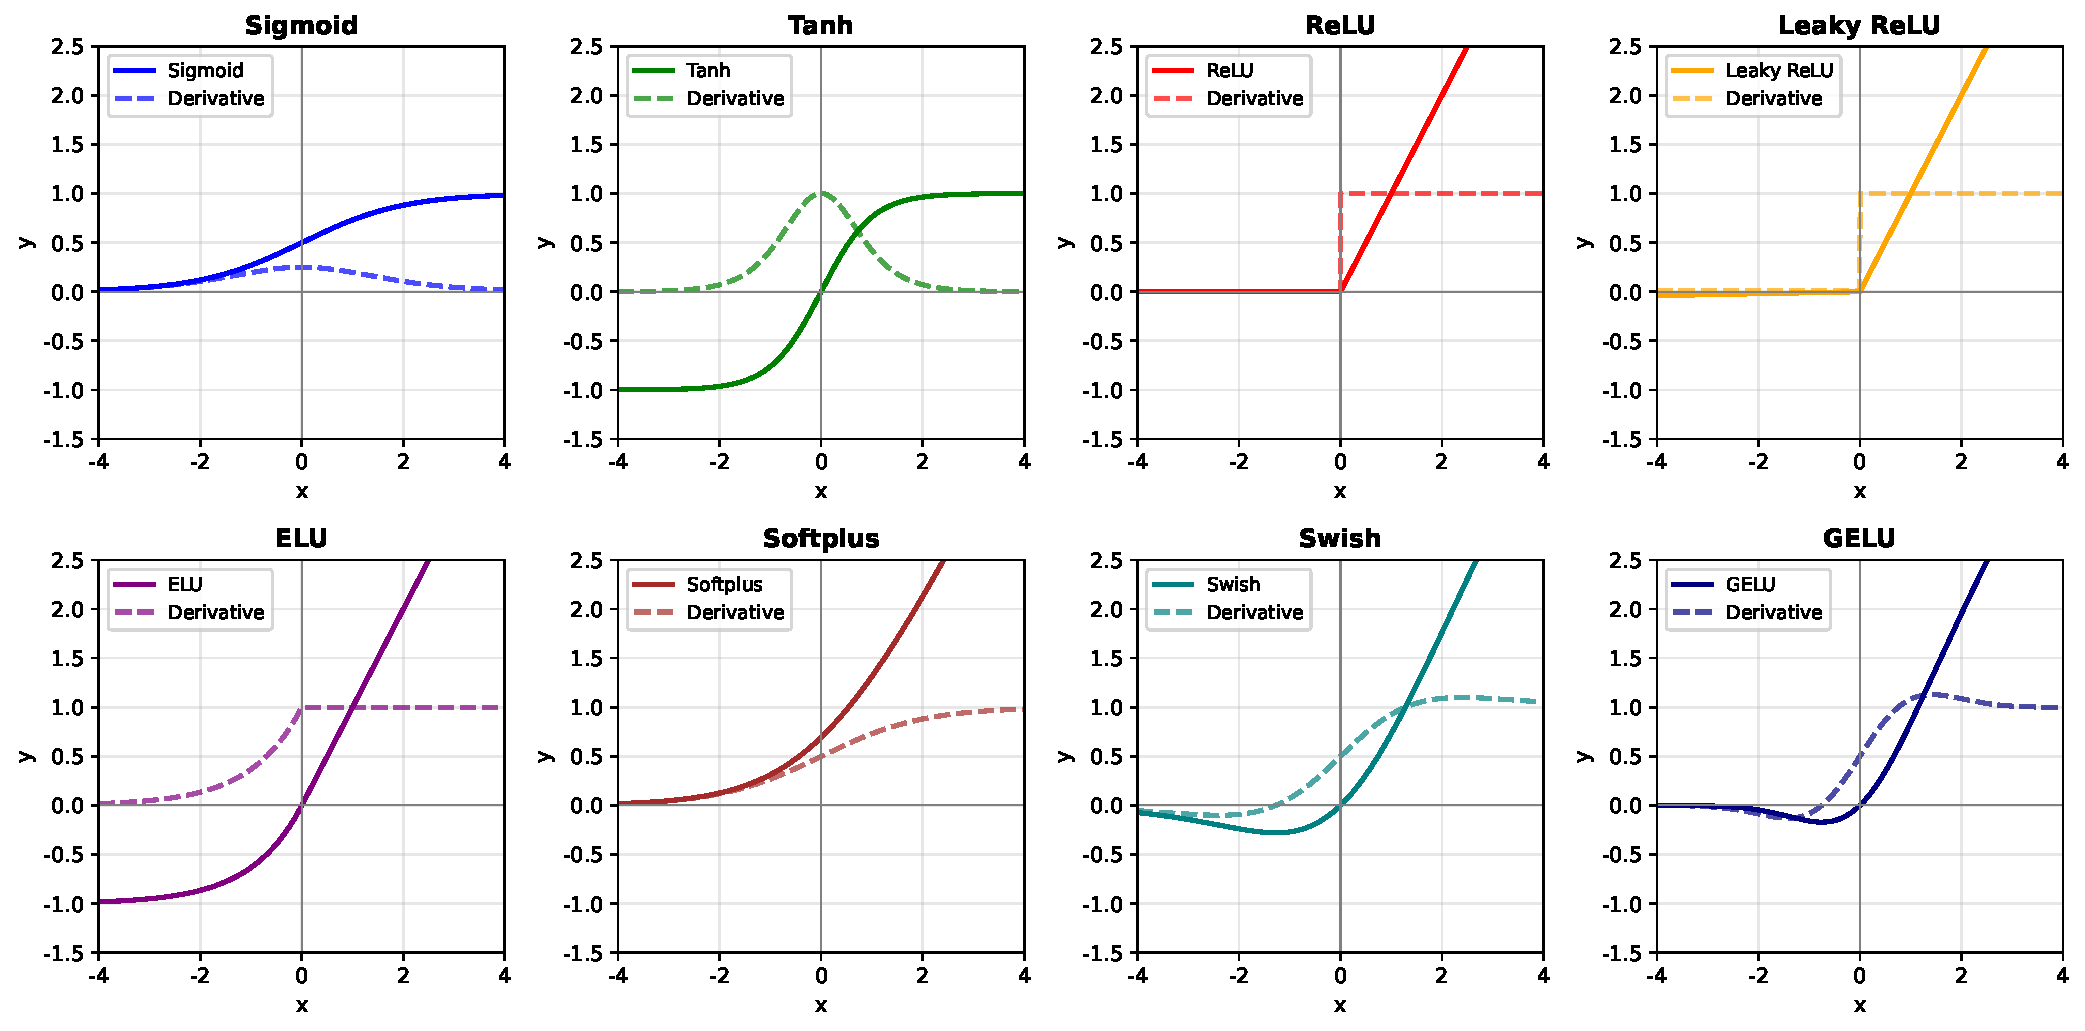
\includegraphics[width=0.95\textwidth]{figs_chap09/activation_functions.pdf}
\caption{常用激活函数（实线）及其导数（虚线）。Sigmoid和Tanh在输入绝对值较大时趋于饱和，导数接近0。ReLU在负半轴完全为0，正半轴导数恒为1。Leaky ReLU、ELU、Swish、GELU都是对ReLU的改进。}
\label{fig:activation_functions}
\end{figure}

\begin{itemize}
    \item \textbf{Sigmoid和Tanh}：输出被"压缩"到有限区间（$[0,1]$或$[-1,1]$），这曾被认为符合生物神经元的激活特性。但它们有严重的\textbf{梯度饱和}问题。

    \item \textbf{ReLU}：极其简单——保留正值，置零负值。计算快、不饱和（正半轴），但可能导致"神经元死亡"。

    \item \textbf{改进版ReLU}：Leaky ReLU、ELU在负半轴保留非零梯度；Swish和GELU则是光滑版本，避免了导数的不连续性。
\end{itemize}

\subsection*{二、手写实现：以Sigmoid为例}

Sigmoid函数的实现看似简单，但有数值陷阱：

\begin{lstlisting}[language=Python]
import numpy as np

def sigmoid_naive(x):
    """朴素实现——可能溢出！"""
    return 1 / (1 + np.exp(-x))

def sigmoid_stable(x):
    """数值稳定实现"""
    return np.where(x >= 0,
                    1 / (1 + np.exp(-x)),
                    np.exp(x) / (1 + np.exp(x)))
\end{lstlisting}

当$x$是很大的负数（如$x = -1000$）时，\texttt{np.exp(-x)}会溢出。稳定版本通过分情况处理避免了这个问题。

Sigmoid的导数有一个优雅的形式：
\[
\sigma'(x) = \sigma(x)(1 - \sigma(x))
\]
这意味着我们可以复用前向传播的结果来计算梯度——这正是深度学习框架的做法。

\subsection*{三、梯度消失问题}

为什么Sigmoid在深度网络中表现不佳？看图\ref{fig:gradient_flow}的中图：

\begin{figure}[htbp]
\centering
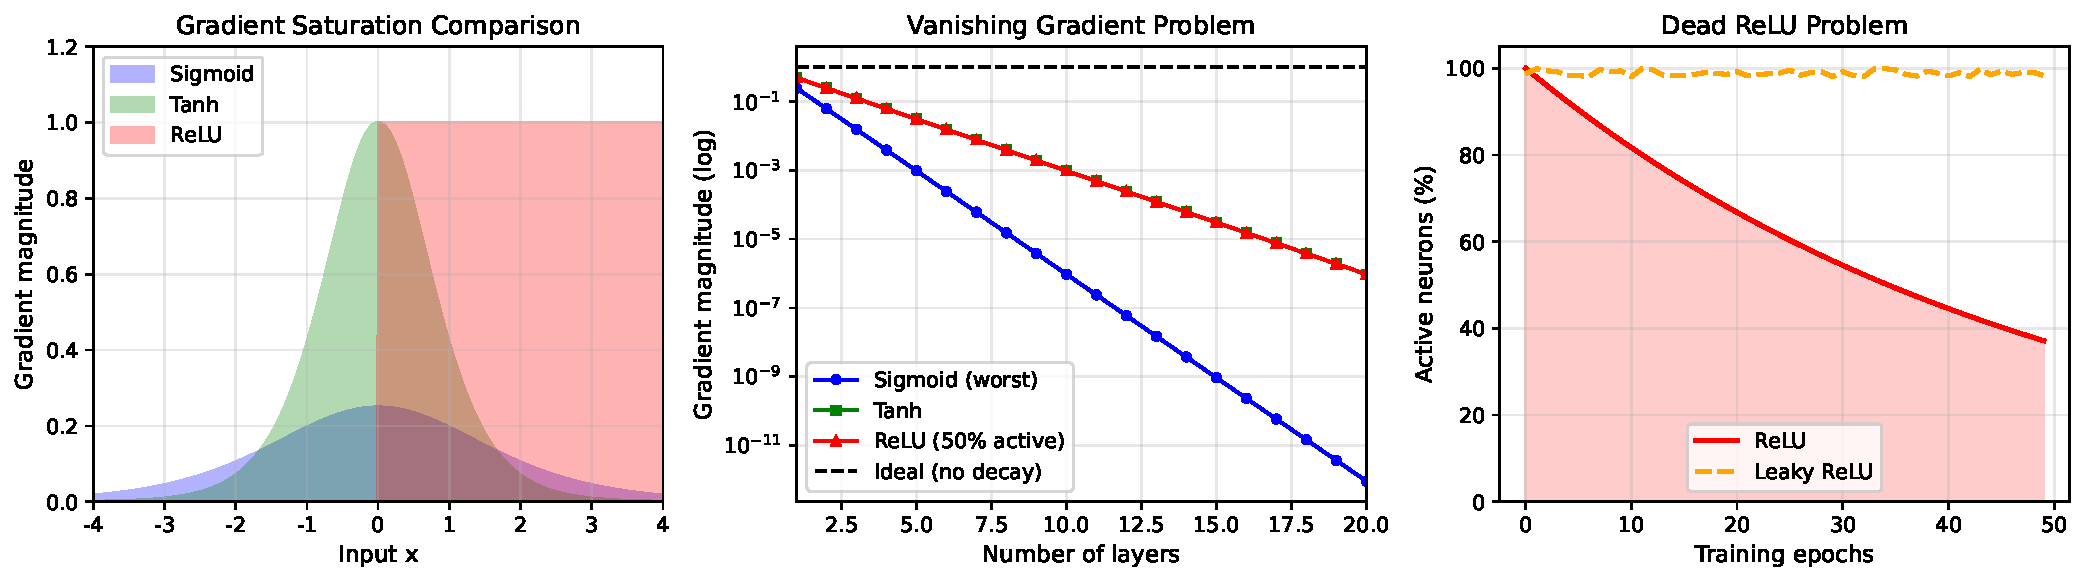
\includegraphics[width=0.95\textwidth]{figs_chap09/gradient_flow.pdf}
\caption{梯度流动分析。左图：不同激活函数的梯度分布。中图：梯度经过多层的衰减（对数尺度）。右图：ReLU的"死亡神经元"问题。}
\label{fig:gradient_flow}
\end{figure}

Sigmoid的最大梯度只有0.25（在$x=0$处）。经过$n$层网络后，梯度最多变成原来的$0.25^n$倍。这就是\textbf{梯度消失}（vanishing gradient）问题——深层网络的参数几乎无法更新。

\marginnote{\textbf{历史注记}：梯度消失问题是神经网络在1990年代陷入低谷的重要原因。直到2006年Hinton等人提出逐层预训练，以及后来ReLU的流行，深度学习才迎来复兴。}

ReLU的优势在于：正半轴的梯度恒为1，不会衰减。这使得梯度可以"无损"地流过任意多层。但ReLU也有代价：负输入的梯度为0，一旦某个神经元进入"死亡"状态，它将永远无法恢复。

\subsection*{四、计算图与反向传播}

理解反向传播的关键是画出\textbf{计算图}（图\ref{fig:computation_graph}）：

\begin{figure}[htbp]
\centering
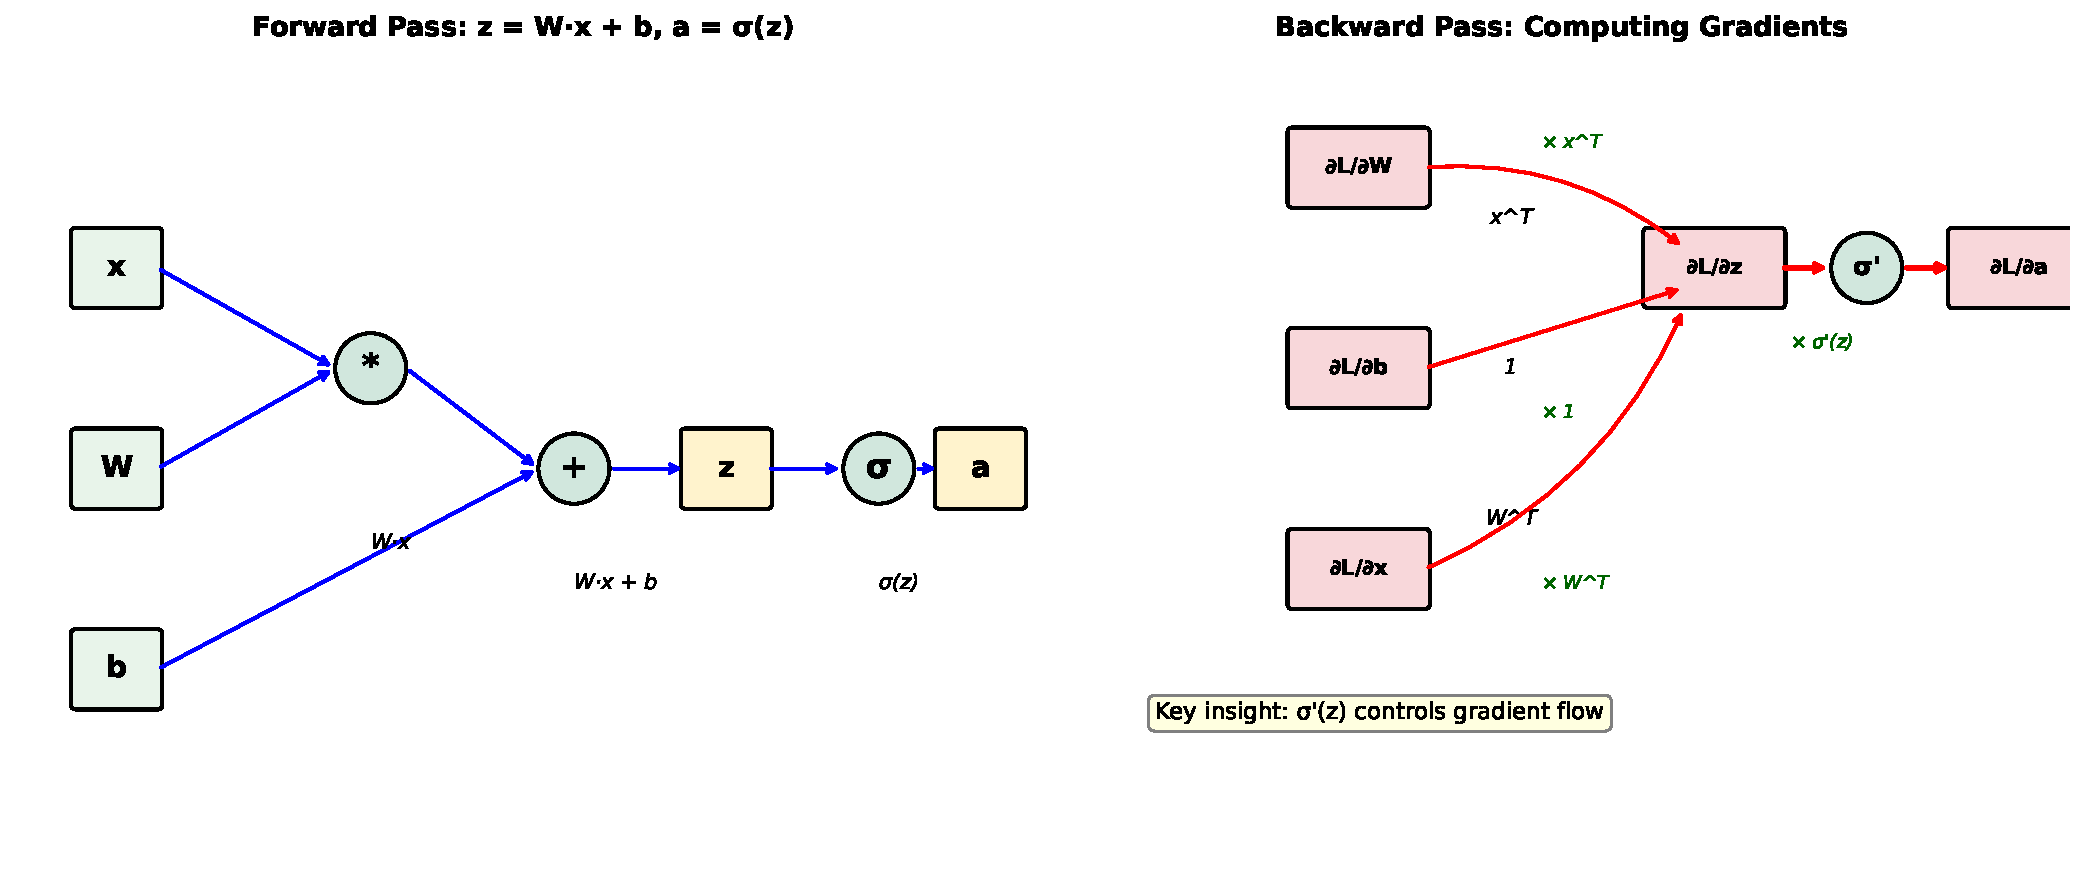
\includegraphics[width=0.95\textwidth]{figs_chap09/computation_graph.pdf}
\caption{单层神经元的计算图。左图：前向传播，从输入$x$计算输出$a$。右图：反向传播，从损失对输出的梯度$\partial L/\partial a$逐步计算对参数$W, b$的梯度。注意$\sigma'(z)$是"阀门"，控制梯度能否有效流回。}
\label{fig:computation_graph}
\end{figure}

前向传播中，信息从左到右流动：$x \to z = Wx+b \to a = \sigma(z)$。

反向传播中，梯度从右到左流动。关键公式是\textbf{链式法则}：
\[
\frac{\partial L}{\partial W} = \frac{\partial L}{\partial a} \cdot \frac{\partial a}{\partial z} \cdot \frac{\partial z}{\partial W} = \frac{\partial L}{\partial a} \cdot \sigma'(z) \cdot x^T
\]

这里$\sigma'(z)$扮演着"阀门"的角色：如果它很小，梯度就流不过去。这解释了为什么激活函数的选择如此重要。

\subsection*{五、梯度检验：验证你的实现}

如何确保手写的梯度公式正确？使用\textbf{数值梯度}验证：
\[
\frac{\partial f}{\partial x} \approx \frac{f(x + \epsilon) - f(x - \epsilon)}{2\epsilon}
\]

图\ref{fig:gradient_check}展示了解析梯度与数值梯度的对比：

\begin{figure}[htbp]
\centering
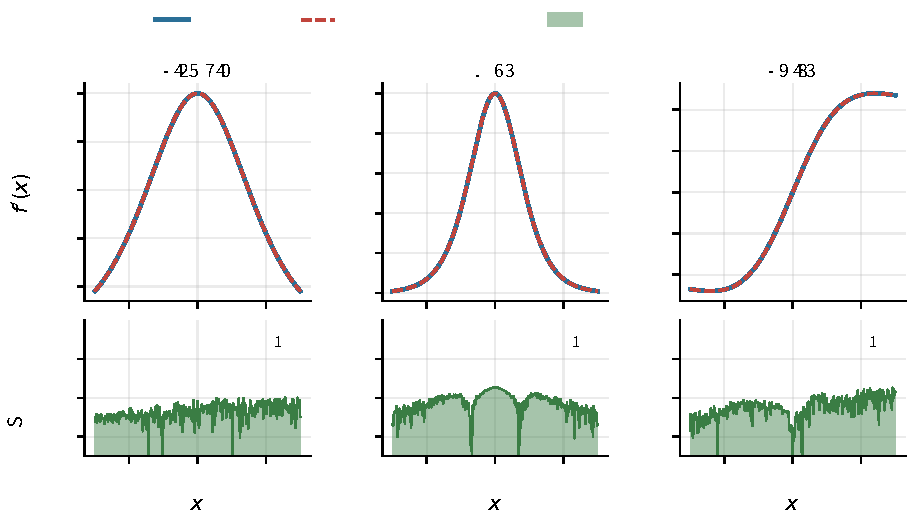
\includegraphics[width=0.95\textwidth]{figs_chap09/gradient_check.pdf}
\caption{梯度检验：解析梯度（蓝色实线）与数值梯度（红色虚线）几乎完全重合。绿色区域显示误差，最大约为$10^{-10}$量级，验证了实现的正确性。}
\label{fig:gradient_check}
\end{figure}

\begin{lstlisting}[language=Python]
def gradient_check(func, deriv, x, eps=1e-5):
    """梯度检验"""
    analytical = deriv(x)
    numerical = (func(x + eps) - func(x - eps)) / (2 * eps)
    error = np.abs(analytical - numerical)
    return error
\end{lstlisting}

如果误差超过$10^{-5}$，很可能你的解析梯度有bug。

\subsection*{六、现代激活函数：GELU与Swish}

GPT和BERT等大模型为什么选择GELU（Gaussian Error Linear Unit）？

\begin{figure}[htbp]
\centering
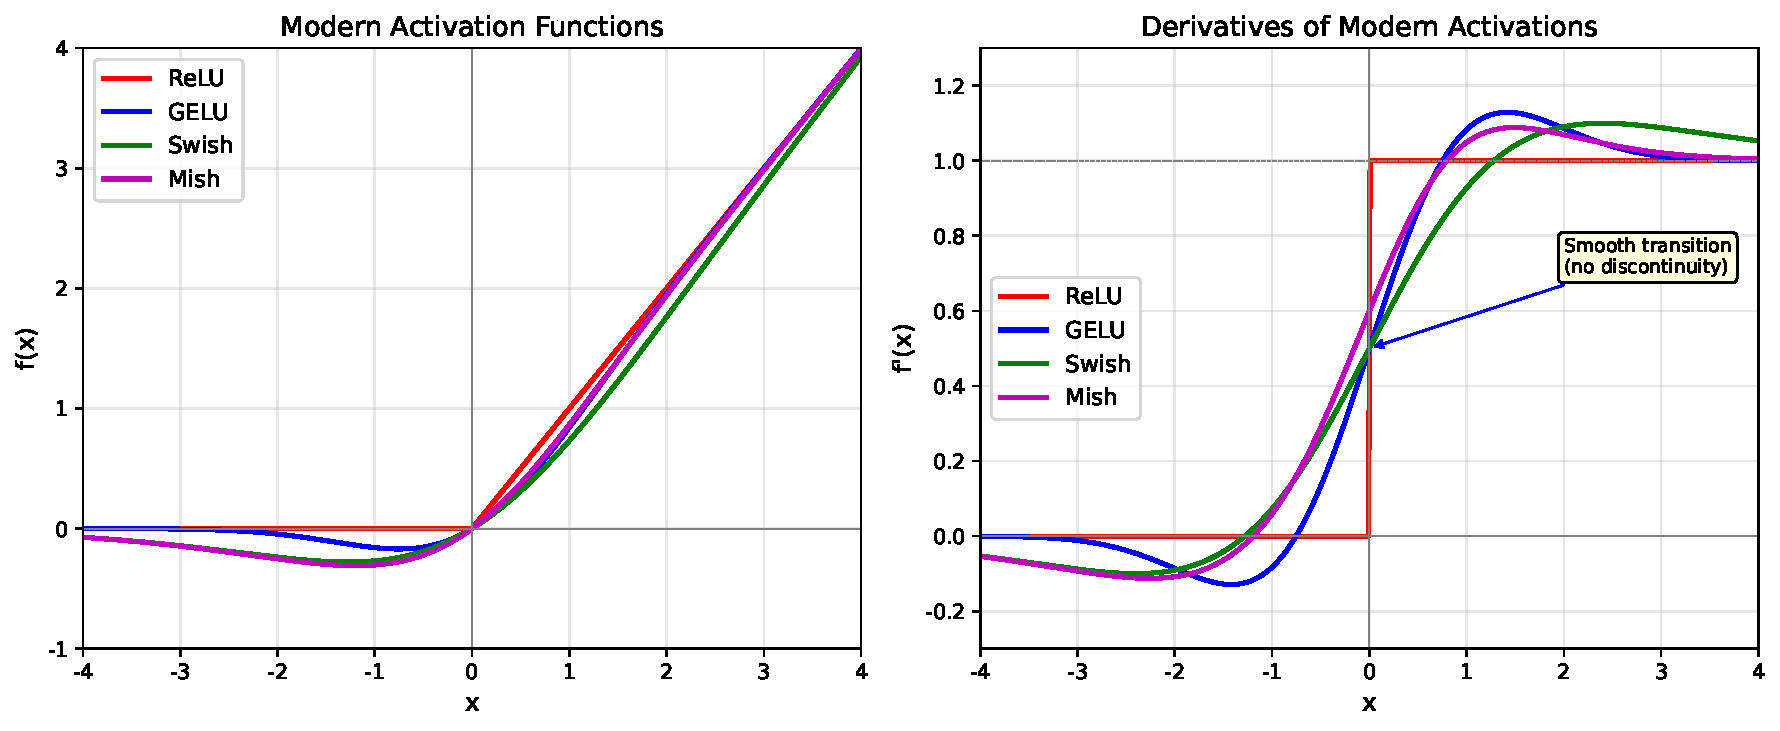
\includegraphics[width=0.9\textwidth]{figs_chap09/modern_activations.pdf}
\caption{现代激活函数对比。GELU、Swish、Mish都是ReLU的光滑近似，在$x=0$附近没有导数的跳跃。右图显示它们的导数曲线，比ReLU更加平滑。}
\label{fig:modern_activations}
\end{figure}

GELU的定义：
\[
\text{GELU}(x) = x \cdot \Phi(x) \approx 0.5x\left(1 + \tanh\left[\sqrt{\frac{2}{\pi}}\left(x + 0.044715x^3\right)\right]\right)
\]
其中$\Phi(x)$是标准正态分布的CDF。

直觉：GELU对输入$x$进行"随机门控"——输入越大，通过的概率越高。这可以看作对dropout的可微近似。

Swish则更简单：$\text{Swish}(x) = x \cdot \sigma(x)$。

这些光滑激活函数的优势：
\begin{itemize}
    \item 导数处处连续，优化过程更稳定
    \item 负半轴不完全为0，避免神经元死亡
    \item 在大规模模型上的实验效果略优于ReLU
\end{itemize}

\subsection*{七、手写自动微分}

最后，我们展示如何用50行代码实现支持激活函数的自动微分：

\begin{lstlisting}[language=Python]
class Tensor:
    def __init__(self, data):
        self.data = data
        self.grad = 0
        self._backward = lambda: None
        self._prev = set()

    def sigmoid(self):
        s = 1 / (1 + np.exp(-self.data))
        out = Tensor(s)
        out._prev = {self}
        def _backward():
            self.grad += s * (1 - s) * out.grad  # 链式法则！
        out._backward = _backward
        return out

    def backward(self):
        # 拓扑排序
        topo = []
        visited = set()
        def build_topo(v):
            if v not in visited:
                visited.add(v)
                for child in v._prev:
                    build_topo(child)
                topo.append(v)
        build_topo(self)

        # 反向传播
        self.grad = 1
        for v in reversed(topo):
            v._backward()
\end{lstlisting}

核心思想：每个操作（如Sigmoid）都记录"如何把输出的梯度传递给输入"。反向传播时，按拓扑逆序依次调用这些函数。

完整代码见\texttt{code\_chap09/activation\_functions.py}。

\subsection*{八、设计哲学小结}

激活函数的演化体现了深度学习的工程智慧：

\begin{enumerate}
    \item \textbf{生物启发 → 数学便利}：Sigmoid模拟神经元激活概率，但数学性质不好。ReLU虽不生物，但训练效果好。

    \item \textbf{简单 → 光滑}：ReLU计算快但不连续，GELU光滑但计算稍贵。在大模型时代，光滑性带来的稳定性更重要。

    \item \textbf{理论 → 实验}：没有任何理论证明GELU一定比ReLU好。选择激活函数更多靠实验调参。
\end{enumerate}

\begin{insightbox}[title=实践建议]
\begin{itemize}
    \item \textbf{默认选ReLU}：简单、快、效果好
    \item \textbf{大模型用GELU}：GPT/BERT的标配
    \item \textbf{遇到"死神经元"换Leaky ReLU}：负半轴保留梯度
    \item \textbf{不确定就实验}：在你的任务上跑几个对比
\end{itemize}
\end{insightbox}

%======================================================================
\section*{扩展阅读：为什么不能随便选择神经网络架构}
\addcontentsline{toc}{section}{扩展阅读：神经网络架构选择}
%======================================================================

神经网络通常被写成一个参数化函数
\[
f_\theta : \mathcal{X} \to \mathcal{Y},
\]
其中 $\theta$ 是网络的所有参数（权重与偏置）。给定一个输入 $x\in\mathcal{X}$，网络输出 $f_\theta(x)$ 作为预测或表示。

不同的网络结构，对 $f_\theta$ 所在的函数集合施加了不同的约束：
\[
\mathcal{F}_{\text{MLP}} \neq \mathcal{F}_{\text{CNN}} \neq \mathcal{F}_{\text{RNN}} \neq \mathcal{F}_{\text{Transformer}} \neq \mathcal{F}_{\text{GNN}}.
\]
这里的 $\mathcal{F}$ 可以理解为"在有限参数规模与有限深度下，网络实际能够高效表示的函数类"。

虽然多层感知机（MLP）在理论上具有通用逼近能力，可以逼近任意连续函数，但在有限宽度、有限深度和有限训练样本的条件下，不同结构对不同类型数据的表达效率差异巨大。本节从公式与直觉两方面，分析典型网络结构与数据结构之间的对应关系，并给出一些"某一结构难以识别、另一结构容易识别"的具体例子。

%----------------------------------------------------------------------
\subsection*{一、基本单元：仿射变换与非线性}
%----------------------------------------------------------------------

\paragraph{单个神经元的计算形式}

最基本的神经元对输入向量 $x\in\mathbb{R}^d$ 的计算为
\[
y = \sigma(w^\top x + b),
\]
其中 $w\in\mathbb{R}^d$ 为权重向量，$b\in\mathbb{R}$ 为偏置，$\sigma(\cdot)$ 为非线性激活函数（如 ReLU, Sigmoid 等）。

几何意义上，$w^\top x + b = 0$ 表示 $\mathbb{R}^d$ 中的一个超平面。对于二分类任务，若将输出二值化：
\[
\hat{y} = \begin{cases} 1, & \sigma(w^\top x + b) \ge \tau,\\ 0, & \text{否则}, \end{cases}
\]
该神经元实质上实现了一个线性分类器，决策边界是一个超平面。

\paragraph{单隐层前馈网络}

一个含单隐层，宽度为 $m$ 的前馈神经网络可以写成
\[
f(x) = \sum_{i=1}^m \alpha_i \,\sigma(w_i^\top x + b_i) + c,
\]
其中 $w_i, b_i$ 为第 $i$ 个隐层神经元的参数，$\alpha_i, c$ 为输出层的参数。

此类网络在理论上满足通用逼近定理：当 $m\to\infty$ 时，在 mild 条件下可以逼近任意连续函数。然而，在固定宽度 $m$ 下，能方便表示的函数仍有强烈结构性。不同的网络结构可以被视为在以下几个方面作出不同的"工程性假设"：

\begin{itemize}
\item 输入特征之间是否存在空间或拓扑结构；
\item 函数是否具有平移、旋转或其他对称性；
\item 是否存在时间或序列依赖；
\item 是否存在图结构（节点与边）约束。
\end{itemize}

后续各节将围绕这些问题展开。

%----------------------------------------------------------------------
\subsection*{二、线性可分性与 XOR：一层网络的能力极限}
%----------------------------------------------------------------------

\paragraph{线性可分与决策边界}

考虑二分类问题，输入 $x\in\mathbb{R}^2$，输出 $y\in\{0,1\}$。若存在某个 $(w,b)$ 使得
\[
w^\top x + b > 0 \Rightarrow y=1,\quad w^\top x + b < 0 \Rightarrow y=0,
\]
则称该数据集合 \emph{线性可分}。此时仅用一个神经元即可实现完美分类，决策边界是平面（在二维即直线）。

若数据不是线性可分，则单个神经元无论如何调整 $w,b$ 都不可能实现零训练误差。这种情况需要多个神经元组合，利用非线性叠加构造更复杂的边界。

\paragraph{XOR 示例：典型的非线性可分问题}

考虑逻辑异或运算 XOR：
\[
\text{XOR}(x_1,x_2) = \begin{cases} 1, & x_1 \ne x_2,\\ 0, & x_1 = x_2. \end{cases}
\]
对应的四个输入--输出对为：
\[
(0,0)\to 0,\quad (1,1)\to 0,\quad (1,0)\to 1,\quad (0,1)\to 1.
\]

将这些点画在二维平面上，可以观察到：

\begin{itemize}
\item $(0,0)$ 与 $(1,1)$ 属于一类；
\item $(1,0)$ 与 $(0,1)$ 属于另一类；
\item 无论怎样画一条直线，都无法将这两类点完全分开。
\end{itemize}

因此 XOR 数据不是线性可分的。一层感知机的决策边界为 $w_1x_1 + w_2x_2 + b = 0$，只能得到一条直线，即只能表示线性可分类。故一层网络无法表示 XOR 函数。

\paragraph{两层网络如何表示 XOR}

引入一个含两个隐含神经元的网络：
\[
h_1 = \sigma(w_1^\top x + b_1), \quad h_2 = \sigma(w_2^\top x + b_2), \quad f(x) = \sigma(\alpha_1 h_1 + \alpha_2 h_2 + c).
\]

可以构造如下形式（用 Heaviside 函数 $H$ 直观说明）：
\[
h_1 = H(x_1 - x_2),\quad h_2 = H(x_2 - x_1).
\]
此时
\[
h_1 = \begin{cases} 1, & x_1 > x_2,\\ 0, & \text{否则}, \end{cases} \quad h_2 = \begin{cases} 1, & x_2 > x_1,\\ 0, & \text{否则}. \end{cases}
\]
对 XOR 的四个点：
\[
\begin{aligned}
(0,0): &\quad h_1=0,\ h_2=0,\\
(1,1): &\quad h_1=0,\ h_2=0,\\
(1,0): &\quad h_1=1,\ h_2=0,\\
(0,1): &\quad h_1=0,\ h_2=1.
\end{aligned}
\]
可以令输出层为
\[
f(x) = H(h_1 + h_2 - 0.5),
\]
则恰好得到 XOR。这里两层结构将平面划分为多个线性区域，再通过线性组合与非线性得到非线性决策边界。

这个例子说明：即使有非线性激活，一层结构的表达能力仍严格受限，只能表示线性可分问题。增加一层后，决策边界可以组合多个线性片段，从而表示更复杂模式。

%----------------------------------------------------------------------
\subsection*{三、卷积网络与局部结构：为什么 CNN 在图像上高效}
%----------------------------------------------------------------------

\paragraph{图像的局部相关性与平移等变性}

将灰度图像视为矩阵 $X \in \mathbb{R}^{H\times W}$，每个像素 $X_{i,j}$ 与其邻近像素在空间上高度相关。许多模式（边缘、角点、纹理）具有以下特征：

\begin{itemize}
\item \textbf{局部性}：可以仅通过一个小邻域（例如 $3\times 3$）来判断；
\item \textbf{平移等变性}：同一个局部模式出现在图像的不同位置时，其语义一致。
\end{itemize}

将这两点作为假设，可以构造卷积神经网络。

\paragraph{卷积运算的形式}

以二维卷积为例，给定卷积核 $K\in\mathbb{R}^{k\times k}$，卷积运算为
\[
(Y = K * X)_{i,j} = \sum_{u=-r}^r \sum_{v=-r}^r K_{u,v}\, X_{i+u, j+v},
\]
其中 $k = 2r+1$。该公式反映两点重要性质：

\begin{itemize}
\item \textbf{局部感受野}：输出 $Y_{i,j}$ 只依赖于输入中 $(i,j)$ 附近的像素；
\item \textbf{权重共享}：同一个卷积核 $K$ 在整张图像上平移使用。
\end{itemize}

若将图像展开为向量 $x\in\mathbb{R}^{HW}$，则卷积对应一个稀疏矩阵 $W_{\text{conv}}$：
\[
\text{vec}(Y) = W_{\text{conv}}\, \text{vec}(X),
\]
其中 $W_{\text{conv}}$ 的非零结构体现了局部连接和权重共享。

与之对比，如果使用全连接层：
\[
y = W_{\text{fc}}\, \text{vec}(X) + b,
\]
矩阵 $W_{\text{fc}}$ 为稠密矩阵，需要 $O(H^2 W^2)$ 个参数，既不利用局部性，也不利用平移不变性；卷积核则只需 $k^2$ 个参数。

\paragraph{边缘检测示例：卷积核的优势}

考虑一幅 $5\times 5$ 的简化图像，包含一条水平边缘：
\[
X = \begin{bmatrix} 1 & 1 & 1 & 1 & 1\\ 1 & 1 & 1 & 1 & 1\\ 0 & 0 & 0 & 0 & 0\\ 0 & 0 & 0 & 0 & 0\\ 0 & 0 & 0 & 0 & 0 \end{bmatrix}.
\]

定义一个垂直边缘检测的卷积核（Sobel 样式）：
\[
K = \begin{bmatrix} 1 & 0 & -1\\ 1 & 0 & -1\\ 1 & 0 & -1 \end{bmatrix}.
\]

对 $X$ 做卷积，局部窗口中亮度差显著处（即边缘）会产生较大响应。卷积核不需要知道边缘出现在图像哪里，只要局部模式相同，响应便相同，这体现了平移等变性。

若用全连接层来手动"学习"边缘检测，则需要为每个可能的边缘位置学习一组单独参数，参数量极大，并且难以泛化到未见过的位置。卷积核通过共享参数，在整个图像上复用同一模式检测器。

\paragraph{从函数类角度的对比}

全连接网络可以表示的线性映射集合为所有 $HW \times HW$ 的矩阵；卷积网络可以表示的线性映射集合仅是其中满足"Toeplitz 块结构"的一小部分。形式上：
\[
\mathcal{L}_{\text{conv}} \subset \mathcal{L}_{\text{fc}}.
\]

这一"缩小函数空间"的操作相当于引入明显且符合图像物理结构的归纳偏置，使得在相同参数规模下，卷积网络在图像任务上能够更高效地拟合正确映射。

%----------------------------------------------------------------------
\subsection*{四、序列建模：RNN 与 Transformer 对长依赖的处理}
\preview{第11章会专门推导 RNN 的梯度消失（把本章的伴随方程沿时间展开）并介绍 Transformer 的注意力机制；这里只从"函数类"的角度做个预告。}
%----------------------------------------------------------------------

\paragraph{RNN 的递推结构}

给定一个长度为 $T$ 的序列 $(x_1, x_2, \dots, x_T)$，循环神经网络（RNN）定义隐状态递推为：
\[
h_t = \phi(W_h h_{t-1} + W_x x_t + b),
\]
输出为
\[
y_t = \psi(W_y h_t + c).
\]

这里 $h_t$ 可以视为对前 $t$ 个输入的"压缩记忆"。理论上，$h_t$ 包含所有历史信息：
\[
h_t = F(x_1, x_2, \dots, x_t).
\]

然而在实践中，由于链式乘积的存在，参数学习会面临梯度消失或爆炸问题。

\paragraph{梯度消失的简要分析}

以损失 $L$ 对某一时刻状态 $h_t$ 的梯度为例：
\[
\frac{\partial L}{\partial h_t} = \frac{\partial L}{\partial h_T} \prod_{k=t+1}^{T} \frac{\partial h_k}{\partial h_{k-1}}.
\]
若将 $\frac{\partial h_k}{\partial h_{k-1}}$ 近似写作某个矩阵 $J_k$，则
\[
\left|\frac{\partial L}{\partial h_t}\right| \le \left|\frac{\partial L}{\partial h_T}\right| \cdot \prod_{k=t+1}^{T} \|J_k\|.
\]
如果 $\|J_k\| < 1$，则该乘积随着 $T-t$ 增大会快速趋向 0，造成梯度消失，从而较难捕获长距离依赖；若 $\|J_k\| > 1$，则会出现梯度爆炸。

LSTM、GRU 等结构通过门控机制缓解这一问题，但根本上仍基于顺序递推。

\paragraph{长依赖示例：远距离一致性}

考虑一个简化任务：输入为括号序列，如
\[
\texttt{( ( ) ( ( ) ) )},
\]
任务是判断括号是否匹配。判断最后一个右括号是否匹配，需要考虑整个序列的结构信息。

RNN 需要在 $h_t$ 中长期保存栈式信息，且训练时梯度需要通过长链传播，容易出现训练困难。在理论上，足够大的 RNN 可以模拟栈机，但在有限参数和梯度下降的训练机制下，学习到稳定的栈行为非常困难。

\paragraph{Transformer 的自注意力机制}

Transformer 使用自注意力机制（self-attention）直接让每个位置与全序列交互。对长度为 $T$ 的序列，先通过线性变换得到
\[
Q = X W_Q,\quad K = X W_K,\quad V = X W_V,
\]
其中 $X\in\mathbb{R}^{T\times d}$ 为输入序列表示，$Q,K,V\in\mathbb{R}^{T\times d_k}$。

自注意力输出为
\[
\text{Attn}(Q,K,V) = \text{softmax}\left(\frac{QK^\top}{\sqrt{d_k}}\right)V.
\]

其中 $(QK^\top)_{ij} = q_i^\top k_j$ 表示位置 $i$ 对位置 $j$ 的相关性。对于每个位置 $i$：
\[
\tilde{h}_i = \sum_{j=1}^{T} \alpha_{ij} v_j,\quad \alpha_{ij} = \frac{\exp(q_i^\top k_j / \sqrt{d_k})}{\sum_{l=1}^{T} \exp(q_i^\top k_l / \sqrt{d_k})}.
\]

这种结构的关键特点是：\emph{任意两个位置之间可以通过单层注意力直接建立联系}，不需要经过多步递推。对于前面的括号任务，某个位置可以直接"关注"与之匹配的括号位置，因此在函数表达上更适合建模远距离依赖。

\paragraph{从函数表达角度的对比}

RNN 所表达的函数类通过递推定义：
\[
h_t = F(h_{t-1}, x_t),
\]
而 Transformer 的自注意力层本质上表达了"任意位置两两交互"的函数：
\[
\tilde{h}_i = G\left(\{x_j\}_{j=1}^{T}\right),
\]
且 $G$ 在构造上具有对位置重排的某些对称性（通过位置编码调节）。从函数空间角度看，Transformer 引入的自注意力操作扩展了对非局部依赖的直接表达能力，使得在有限深度下更容易表示需要远距离交互的函数。

%----------------------------------------------------------------------
\subsection*{五、图结构数据与图神经网络}
%----------------------------------------------------------------------

\paragraph{图结构数据的特征}

图 $G = (V, E)$ 由节点集合 $V$ 与边集合 $E$ 组成。典型例子包括：

\begin{itemize}
\item 社交网络：节点为用户，边为好友关系；
\item 交通网络：节点为路口或站点，边为道路或轨道；
\item 电力网络：节点为变电站或母线，边为输电线路；
\item 分子结构：节点为原子，边为化学键。
\end{itemize}

图数据的重要特征在于：拓扑结构本身承载了关键信息。节点的功能不仅由其自身特征决定，还由其邻居及更远节点的结构关系决定。

\paragraph{图神经网络的消息传递框架}

图神经网络（Graph Neural Network, GNN）的一个典型形式是消息传递神经网络（Message Passing Neural Network, MPNN）。在第 $k$ 层，第 $i$ 个节点特征更新规则为：
\[
h_i^{(k+1)} = \phi\Big(h_i^{(k)},\ \square_{j\in\mathcal{N}(i)} \psi\big(h_i^{(k)}, h_j^{(k)}, e_{ij}\big)\Big),
\]
其中
\begin{itemize}
\item $h_i^{(k)}$ 为节点 $i$ 在第 $k$ 层的表示；
\item $\mathcal{N}(i)$ 为节点 $i$ 的邻居集合；
\item $e_{ij}$ 为边 $(i,j)$ 的特征；
\item $\psi$ 为消息函数，$\phi$ 为更新函数；
\item $\square$ 为一个置换不变的聚合算子（如求和、平均或最大）。
\end{itemize}

该形式体现了图结构的两个关键性质：

\begin{itemize}
\item \textbf{局部性}：节点表示由邻居的表示聚合而来；
\item \textbf{置换不变性}：邻居节点顺序可以任意变换，不影响聚合结果。
\end{itemize}

\paragraph{图结构上 CNN 的局限}

若尝试将普通 CNN 直接应用于图，存在若干困难：

\begin{itemize}
\item 图通常是非规则结构，不存在自然的二维网格坐标 $(i,j)$；
\item 不同节点的度数不同，难以定义固定形状的"卷积核邻域"；
\item 图结构不存在平移对称性，不能简单依赖权重共享在规则网格上的平移。
\end{itemize}

因此，传统卷积无法直接刻画图上的邻接关系与拓扑属性。而 GNN 通过邻居聚合的形式，将图的邻接结构内置到更新规则中。例如，一阶 GCN（Graph Convolutional Network）层可写作：
\[
H^{(k+1)} = \sigma\left(\tilde{D}^{-1/2} \tilde{A} \tilde{D}^{-1/2} H^{(k)} W^{(k)}\right),
\]
其中 $\tilde{A} = A + I$ 为加入自环的邻接矩阵，$\tilde{D}$ 为对应度矩阵，$H^{(k)}$ 为所有节点的表示矩阵。该结构利用了图拉普拉斯算子的谱特性，从谱图论角度实现了"图上的卷积"。

\paragraph{拓扑敏感任务中的结构差异}

考虑以下任务：给定电力网络拓扑与各节点负荷，预测某条线路是否存在过载风险。该任务的输出不仅取决于某条线的局部属性，还取决于整个网络的潮流分布。

若将网络拓扑展开为某种顺序向量输入全连接网络，理论上可以表达正确函数，但需要网络在训练中"重新学会"图的拓扑结构与 Kirchhoff 定律之类的物理约束，学习效率低。而 GNN 在结构上即按照图拓扑传播与聚合信息，更接近实际物理过程，因此在相同参数规模下更容易学习到合理函数。

%----------------------------------------------------------------------
\subsection*{六、函数空间与归纳偏置}
%----------------------------------------------------------------------

\paragraph{通用逼近与有效逼近}

多层感知机的通用逼近定理表明：对于紧致集合上的任意连续函数 $f$，存在一个宽度足够的大单隐层网络，使得
\[
\sup_{x\in K} |f(x) - f_\theta(x)| < \varepsilon
\]
对任意 $\varepsilon>0$ 成立。

然而该定理没有给出网络宽度、参数规模与逼近误差之间的有效关系，也没有考虑训练算法与数据分布。实际中更关心的问题是：在给定参数预算与数据规模下，哪类结构能够"高效"表示目标函数。

\paragraph{结构约束下的函数类}

可以将不同结构的网络理解为在参数空间 $\Theta$ 上施加不同的结构约束，从而改变可表达函数集：
\[
\mathcal{F} = \{f_\theta : \theta\in\Theta\}.
\]

\begin{itemize}
\item 对于全连接网络，$\Theta_{\text{fc}}$ 包含所有稠密矩阵参数，$\mathcal{F}_{\text{fc}}$ 十分宽泛；
\item 对于卷积网络，$\Theta_{\text{conv}}$ 仅包含卷积核参数，且强制权重共享，$\mathcal{F}_{\text{conv}}$ 是 $\mathcal{F}_{\text{fc}}$ 的一个子集；
\item 对于 RNN/Transformer/GNN，$\Theta$ 中都包含特定形式的权重共享、对称性或拓扑约束。
\end{itemize}

这些约束可以被视为归纳偏置（inductive bias）：在函数空间中优先选择满足某些不变性或等变性的函数。例如：

\begin{itemize}
\item 卷积层偏向选择平移等变函数；
\item GNN 偏向选择在节点重标号下保持不变的图函数；
\item 自注意力层偏向选择依赖于 token 间相对相似性的函数。
\end{itemize}

\paragraph{对称性与等变性}

设有一组变换构成的群 $G$（例如图像的平移群）。若函数 $f$ 满足
\[
f(T_g x) = f(x),\quad \forall g\in G,
\]
称 $f$ 对 $G$ 不变；若满足
\[
f(T_g x) = T'_g f(x),
\]
称 $f$ 对 $G$ 等变。卷积网络通过局部感受野与权重共享，实现了对平移的等变性；池化操作进一步导致对平移的不变性。

\paragraph{归纳偏置与数据结构匹配}

当数据的真实生成机制具有某种对称性或结构时，将相同的结构内置到网络中，可以显著减少所需参数与训练样本。相反，若选择与数据结构不匹配的网络结构，则需要更多参数、更多数据才能"在函数空间中搜索到"合适的函数，甚至在有限资源下根本难以学到。

从这个角度看，不同架构的"适用领域"可以概括为：

\begin{itemize}
\item MLP：适合无明显空间或拓扑结构的小规模特征；
\item CNN：适合具有局部相关性和平移等变性的网格数据（图像、某些 PDE 网格）；
\item RNN/LSTM：适合中短距离依赖为主的序列；
\item Transformer：适合存在长距离依赖或全局交互的序列与多模态数据；
\item GNN：适合拓扑结构重要、以图为基本对象的数据。
\end{itemize}

%----------------------------------------------------------------------
\subsection*{七、小结}
%----------------------------------------------------------------------

本节从公式与结构出发，讨论了不同神经网络架构与不同类型问题之间的对应关系。主要结论可以概括如下：

\begin{enumerate}
\item 单层网络（线性分类器）只能实现线性可分问题，典型反例是 XOR；增加层数后，通过叠加多个仿射变换与非线性，可以构造更复杂的分段线性决策边界。

\item 卷积网络通过局部感受野与权重共享假设，内置了对平移等变性的归纳偏置，极大提高了在图像等网格结构数据上的表达效率；全连接网络虽然理论上也能表示相同函数，但参数规模与学习难度远大于卷积网络。

\item RNN 通过递推关系建模序列，但梯度需要沿时间方向传播，容易出现梯度消失，难以捕获长距离依赖；Transformer 的自注意力机制允许任意位置之间直接交互，在表达远距离依赖方面更具优势。

\item 图神经网络通过消息传递与邻居聚合机制，将图的拓扑结构直接编码到网络更新规则中，适合处理社交网络、电网、交通网络等图结构数据；传统 CNN 由于依赖规则网格和平移对称性，难以直接应用于一般图。

\item 从函数空间与归纳偏置的角度看，不同架构对应不同的可表达函数类。通过引入与数据生成机制相匹配的结构性假设，可以在有限参数和样本条件下，更高效地学习到合理的函数映射。
\end{enumerate}

在具体应用中，网络结构的选择可以被理解为：对数据结构、任务需求与物理或统计规律的一种工程化编码。理解这些结构背后的数学与直观假设，是构建有效深度学习模型的重要基础。